% Options for packages loaded elsewhere
\PassOptionsToPackage{unicode}{hyperref}
\PassOptionsToPackage{hyphens}{url}
%
\documentclass[
]{article}
\usepackage{lmodern}
\usepackage{amsmath}
\usepackage{ifxetex,ifluatex}
\ifnum 0\ifxetex 1\fi\ifluatex 1\fi=0 % if pdftex
  \usepackage[T1]{fontenc}
  \usepackage[utf8]{inputenc}
  \usepackage{textcomp} % provide euro and other symbols
  \usepackage{amssymb}
\else % if luatex or xetex
  \usepackage{unicode-math}
  \defaultfontfeatures{Scale=MatchLowercase}
  \defaultfontfeatures[\rmfamily]{Ligatures=TeX,Scale=1}
\fi
% Use upquote if available, for straight quotes in verbatim environments
\IfFileExists{upquote.sty}{\usepackage{upquote}}{}
\IfFileExists{microtype.sty}{% use microtype if available
  \usepackage[]{microtype}
  \UseMicrotypeSet[protrusion]{basicmath} % disable protrusion for tt fonts
}{}
\makeatletter
\@ifundefined{KOMAClassName}{% if non-KOMA class
  \IfFileExists{parskip.sty}{%
    \usepackage{parskip}
  }{% else
    \setlength{\parindent}{0pt}
    \setlength{\parskip}{6pt plus 2pt minus 1pt}}
}{% if KOMA class
  \KOMAoptions{parskip=half}}
\makeatother
\usepackage{xcolor}
\IfFileExists{xurl.sty}{\usepackage{xurl}}{} % add URL line breaks if available
\IfFileExists{bookmark.sty}{\usepackage{bookmark}}{\usepackage{hyperref}}
\hypersetup{
  pdftitle={Carbonate chemistry at Ny-Ålesund: AWIPEV-CO2 Project},
  pdfauthor={Jean-Pierre Gattuso and Samir Alliouane},
  hidelinks,
  pdfcreator={LaTeX via pandoc}}
\urlstyle{same} % disable monospaced font for URLs
\usepackage[margin=1in]{geometry}
\usepackage{longtable,booktabs}
\usepackage{calc} % for calculating minipage widths
% Correct order of tables after \paragraph or \subparagraph
\usepackage{etoolbox}
\makeatletter
\patchcmd\longtable{\par}{\if@noskipsec\mbox{}\fi\par}{}{}
\makeatother
% Allow footnotes in longtable head/foot
\IfFileExists{footnotehyper.sty}{\usepackage{footnotehyper}}{\usepackage{footnote}}
\makesavenoteenv{longtable}
\usepackage{graphicx}
\makeatletter
\def\maxwidth{\ifdim\Gin@nat@width>\linewidth\linewidth\else\Gin@nat@width\fi}
\def\maxheight{\ifdim\Gin@nat@height>\textheight\textheight\else\Gin@nat@height\fi}
\makeatother
% Scale images if necessary, so that they will not overflow the page
% margins by default, and it is still possible to overwrite the defaults
% using explicit options in \includegraphics[width, height, ...]{}
\setkeys{Gin}{width=\maxwidth,height=\maxheight,keepaspectratio}
% Set default figure placement to htbp
\makeatletter
\def\fps@figure{htbp}
\makeatother
\setlength{\emergencystretch}{3em} % prevent overfull lines
\providecommand{\tightlist}{%
  \setlength{\itemsep}{0pt}\setlength{\parskip}{0pt}}
\setcounter{secnumdepth}{-\maxdimen} % remove section numbering
\ifluatex
  \usepackage{selnolig}  % disable illegal ligatures
\fi

\title{Carbonate chemistry at Ny-Ålesund: AWIPEV-CO\textsubscript{2}
Project}
\author{Jean-Pierre Gattuso and Samir Alliouane}
\date{31 December 2020}

\begin{document}
\maketitle


\includegraphics[width=2.60417in,height=\textheight]{Images/AWIPEV-Logo.jpg}

\hypertarget{section}{%
\section{}\label{section}}

\hypertarget{infos}{%
\subsection{Infos}\label{infos}}

\hypertarget{introduction}{%
\subsubsection{\texorpdfstring{\textbf{Introduction}}{Introduction}}\label{introduction}}

The AWIPEV-CO2 project aims at starting the first time series for the
carbonate chemistry in the Arctic Ocean as part of the AWIPEV Underwater
Observatory. It comprises two components: (1) continuous real-time
measurements and (2) discrete measurements. The rationale is that
discrete measurements are absolutely needed to calibrate and validate
the sensors.

\hypertarget{awipev-underwater-observatory}{%
\subsubsection{\texorpdfstring{\textbf{AWIPEV Underwater
Observatory}}{AWIPEV Underwater Observatory}}\label{awipev-underwater-observatory}}

The AWIPEV Underwater Observatory has been deployed at Ny-Alesund
(Spitsbergen, 78°55'18N, 11°56'31E) in June 2012. It is part of the
German Project COSYNA (Coastal Observation Systems of the Northern- and
Arctic Seas), which aims at increasing the availability of continuous
real-time data from remote but climatically-sensitive ecosystems. The
AWIPEV underwater observatory comprises a fully remote controlled
FerryBox system fed with seawater pumped in front of the old pIer at 12
m depth. Temperature, salinity, pressure, turbidity, oxygen,
chl-\emph{a} fluorescence are measured. Furthermore, an additional
remote controlled underwater sensor unit able to profile from 12 m to
the surface at any frequency carries additional sensors for salinity,
pressure, turbidity, oxygen chl-\emph{a} fluorescence and PAR. The
system also comprises an ADCP for continuous measurements of currents
and waves. Besides these standard sensors, the underwater unit is
equipped with a webcam and stereo-optical device to remotely assess fish
and jellyfish populations. The AWIPEV observatory is specifically
designed for polar experimental work under extreme conditions including
ice coverage and the inaccessibility for about 7 months during polar
winter. During this time, the system is remotely controlled and
maintained from Germany. All data sampled by the sensors are
continuously sent to a central server system at Helgoland Island where
the data are stored and processed. The processed data are open access
and available at \url{http://codm.hzg.de/codm}.

\hypertarget{continuous-and-semi-continuous-measurements}{%
\subsubsection{\texorpdfstring{\textbf{Continuous and semi-continuous
measurements}}{Continuous and semi-continuous measurements}}\label{continuous-and-semi-continuous-measurements}}

The Arctic version of the Contros-Kongsberg HydroC CO\textsubscript{2}
FT (Carbon Dioxyde partial pressure Flow Through surface water sensor)
has been installed in July 2015. Molecules of dissolved
CO\textsubscript{2} diffuse through a thin composite membrane into the
internal gas circuit leading to a detector chamber, where the partial
pressure of CO\textsubscript{2} is determined by means of infra-red
absorption spectrometry. Concentration-dependent IR light is converted
into the output signal from calibration coefficients stored in firmware
and data from additional sensors within the gas circuit. The measuring
range is 200-1000 uatm, resolution is \textless{} 1 uatm and accuracy is
+- 1\% reading. The sensor is the first instrument in the measuring
loop; data are logged every minute. This instrument requires yearly
factory calibration; two sensors ara available to allow a continuous
time series.

Since February 2016, total alkalinity (AT) is measured every 90 min with
a Contros-Kongsberg HydroFIA TA (Total Alkalinity analyser flow through
system). Fifty ml of seawater is filtered (0.2 um) using a
Contros-Kongsberg cross-flow filter and then acidified using dilute
hydrochloric acid (0.1 N). CO\textsubscript{2} is then flushed out
(open-cell titration) and the final pH measured by means of an indicator
dye (bromocresol green) and visible absorption spectrometry. Together
with salinity and temperature at the time of measurement, the pH reading
is used to calculate AT. According to the manufacturer, the measuring
range is 400 umol/kg dynamic range, resolution 0.1 umol/kg, accuracy 25
umol/kg (+- 1\%) and precision 5 umol/kg (+- 0.2\%).

In August 2017, a seaFET Ocean pH sensor (Sea-Bird Scientific) has been
added to the UWO. This new sensor continuously measures pH at 11 m using
an ISFET (Ion Sensitive Field Effect Transistor). According to the
manufacturer, the measuring range is between 6.5 and 9 pH units, initial
accuracy is 0.02 pH units and precision is 0.004 pH units. Operating
salinity and temperature range are 20 to 40 PSU and 0 to 50°C
respectively.

In August 2017, a Durafet III pH electrode connected to a UDA2128
Analyser (Honeywell) was also implemented to the Ferrybox flow-through
system. This electrode continuously measures pH, in the Ferrybox,
through an ISFET. According to the manufacturer, the measuring range is
between 0 and 14 pH units.

\hypertarget{data-availability}{%
\subsubsection{\texorpdfstring{\textbf{Data
availability}}{Data availability}}\label{data-availability}}

The data at one minute frequency were tagged with the following quality
flags

\begin{itemize}
\item
  1: good data
\item
  3: failing the date and time test
\item
  4: data not usable according to manufacturer
\item
  6: failing the manufacturer range test (not used)
\item
  7: failing the regional range test
\item
  12: failing the spike test (NAs from despike)
\item
  13: failing the gradient test
\item
  15: instrument not deployed or operated
\item
  16: acid flush
\item
  99: failing the final visual inspection
\item
  Despike using oce::despike with n=2, k=5761
\end{itemize}

\begin{longtable}[]{@{}lrrrrrrr@{}}
\toprule
\begin{minipage}[b]{(\columnwidth - 7\tabcolsep) * \real{0.05}}\raggedright
Flag\strut
\end{minipage} &
\begin{minipage}[b]{(\columnwidth - 7\tabcolsep) * \real{0.05}}\raggedleft
pCO2\strut
\end{minipage} &
\begin{minipage}[b]{(\columnwidth - 7\tabcolsep) * \real{0.17}}\raggedleft
Salinity FerryBox\strut
\end{minipage} &
\begin{minipage}[b]{(\columnwidth - 7\tabcolsep) * \real{0.16}}\raggedleft
In situ salinity\strut
\end{minipage} &
\begin{minipage}[b]{(\columnwidth - 7\tabcolsep) * \real{0.20}}\raggedleft
Temperature FerryBox\strut
\end{minipage} &
\begin{minipage}[b]{(\columnwidth - 7\tabcolsep) * \real{0.19}}\raggedleft
In situ temperature\strut
\end{minipage} &
\begin{minipage}[b]{(\columnwidth - 7\tabcolsep) * \real{0.10}}\raggedleft
Durafet pH\strut
\end{minipage} &
\begin{minipage}[b]{(\columnwidth - 7\tabcolsep) * \real{0.09}}\raggedleft
seaFET pH\strut
\end{minipage}\tabularnewline
\midrule
\endhead
\begin{minipage}[t]{(\columnwidth - 7\tabcolsep) * \real{0.05}}\raggedright
1\strut
\end{minipage} &
\begin{minipage}[t]{(\columnwidth - 7\tabcolsep) * \real{0.05}}\raggedleft
56.9\strut
\end{minipage} &
\begin{minipage}[t]{(\columnwidth - 7\tabcolsep) * \real{0.17}}\raggedleft
68.2\strut
\end{minipage} &
\begin{minipage}[t]{(\columnwidth - 7\tabcolsep) * \real{0.16}}\raggedleft
51.8\strut
\end{minipage} &
\begin{minipage}[t]{(\columnwidth - 7\tabcolsep) * \real{0.20}}\raggedleft
66.5\strut
\end{minipage} &
\begin{minipage}[t]{(\columnwidth - 7\tabcolsep) * \real{0.19}}\raggedleft
75.1\strut
\end{minipage} &
\begin{minipage}[t]{(\columnwidth - 7\tabcolsep) * \real{0.10}}\raggedleft
76.2\strut
\end{minipage} &
\begin{minipage}[t]{(\columnwidth - 7\tabcolsep) * \real{0.09}}\raggedleft
69.7\strut
\end{minipage}\tabularnewline
\begin{minipage}[t]{(\columnwidth - 7\tabcolsep) * \real{0.05}}\raggedright
4\strut
\end{minipage} &
\begin{minipage}[t]{(\columnwidth - 7\tabcolsep) * \real{0.05}}\raggedleft
2.4\strut
\end{minipage} &
\begin{minipage}[t]{(\columnwidth - 7\tabcolsep) * \real{0.17}}\raggedleft
NA\strut
\end{minipage} &
\begin{minipage}[t]{(\columnwidth - 7\tabcolsep) * \real{0.16}}\raggedleft
NA\strut
\end{minipage} &
\begin{minipage}[t]{(\columnwidth - 7\tabcolsep) * \real{0.20}}\raggedleft
NA\strut
\end{minipage} &
\begin{minipage}[t]{(\columnwidth - 7\tabcolsep) * \real{0.19}}\raggedleft
NA\strut
\end{minipage} &
\begin{minipage}[t]{(\columnwidth - 7\tabcolsep) * \real{0.10}}\raggedleft
NA\strut
\end{minipage} &
\begin{minipage}[t]{(\columnwidth - 7\tabcolsep) * \real{0.09}}\raggedleft
NA\strut
\end{minipage}\tabularnewline
\begin{minipage}[t]{(\columnwidth - 7\tabcolsep) * \real{0.05}}\raggedright
7\strut
\end{minipage} &
\begin{minipage}[t]{(\columnwidth - 7\tabcolsep) * \real{0.05}}\raggedleft
9.3\strut
\end{minipage} &
\begin{minipage}[t]{(\columnwidth - 7\tabcolsep) * \real{0.17}}\raggedleft
0.1\strut
\end{minipage} &
\begin{minipage}[t]{(\columnwidth - 7\tabcolsep) * \real{0.16}}\raggedleft
11.9\strut
\end{minipage} &
\begin{minipage}[t]{(\columnwidth - 7\tabcolsep) * \real{0.20}}\raggedleft
0.1\strut
\end{minipage} &
\begin{minipage}[t]{(\columnwidth - 7\tabcolsep) * \real{0.19}}\raggedleft
0.0\strut
\end{minipage} &
\begin{minipage}[t]{(\columnwidth - 7\tabcolsep) * \real{0.10}}\raggedleft
3.0\strut
\end{minipage} &
\begin{minipage}[t]{(\columnwidth - 7\tabcolsep) * \real{0.09}}\raggedleft
0.2\strut
\end{minipage}\tabularnewline
\begin{minipage}[t]{(\columnwidth - 7\tabcolsep) * \real{0.05}}\raggedright
12\strut
\end{minipage} &
\begin{minipage}[t]{(\columnwidth - 7\tabcolsep) * \real{0.05}}\raggedleft
1.7\strut
\end{minipage} &
\begin{minipage}[t]{(\columnwidth - 7\tabcolsep) * \real{0.17}}\raggedleft
5.3\strut
\end{minipage} &
\begin{minipage}[t]{(\columnwidth - 7\tabcolsep) * \real{0.16}}\raggedleft
NA\strut
\end{minipage} &
\begin{minipage}[t]{(\columnwidth - 7\tabcolsep) * \real{0.20}}\raggedleft
7.0\strut
\end{minipage} &
\begin{minipage}[t]{(\columnwidth - 7\tabcolsep) * \real{0.19}}\raggedleft
7.8\strut
\end{minipage} &
\begin{minipage}[t]{(\columnwidth - 7\tabcolsep) * \real{0.10}}\raggedleft
1.0\strut
\end{minipage} &
\begin{minipage}[t]{(\columnwidth - 7\tabcolsep) * \real{0.09}}\raggedleft
NA\strut
\end{minipage}\tabularnewline
\begin{minipage}[t]{(\columnwidth - 7\tabcolsep) * \real{0.05}}\raggedright
15\strut
\end{minipage} &
\begin{minipage}[t]{(\columnwidth - 7\tabcolsep) * \real{0.05}}\raggedleft
24.6\strut
\end{minipage} &
\begin{minipage}[t]{(\columnwidth - 7\tabcolsep) * \real{0.17}}\raggedleft
26.4\strut
\end{minipage} &
\begin{minipage}[t]{(\columnwidth - 7\tabcolsep) * \real{0.16}}\raggedleft
36.4\strut
\end{minipage} &
\begin{minipage}[t]{(\columnwidth - 7\tabcolsep) * \real{0.20}}\raggedleft
26.4\strut
\end{minipage} &
\begin{minipage}[t]{(\columnwidth - 7\tabcolsep) * \real{0.19}}\raggedleft
17.0\strut
\end{minipage} &
\begin{minipage}[t]{(\columnwidth - 7\tabcolsep) * \real{0.10}}\raggedleft
19.8\strut
\end{minipage} &
\begin{minipage}[t]{(\columnwidth - 7\tabcolsep) * \real{0.09}}\raggedleft
30.0\strut
\end{minipage}\tabularnewline
\begin{minipage}[t]{(\columnwidth - 7\tabcolsep) * \real{0.05}}\raggedright
16\strut
\end{minipage} &
\begin{minipage}[t]{(\columnwidth - 7\tabcolsep) * \real{0.05}}\raggedleft
5.1\strut
\end{minipage} &
\begin{minipage}[t]{(\columnwidth - 7\tabcolsep) * \real{0.17}}\raggedleft
NA\strut
\end{minipage} &
\begin{minipage}[t]{(\columnwidth - 7\tabcolsep) * \real{0.16}}\raggedleft
NA\strut
\end{minipage} &
\begin{minipage}[t]{(\columnwidth - 7\tabcolsep) * \real{0.20}}\raggedleft
NA\strut
\end{minipage} &
\begin{minipage}[t]{(\columnwidth - 7\tabcolsep) * \real{0.19}}\raggedleft
NA\strut
\end{minipage} &
\begin{minipage}[t]{(\columnwidth - 7\tabcolsep) * \real{0.10}}\raggedleft
NA\strut
\end{minipage} &
\begin{minipage}[t]{(\columnwidth - 7\tabcolsep) * \real{0.09}}\raggedleft
NA\strut
\end{minipage}\tabularnewline
\begin{minipage}[t]{(\columnwidth - 7\tabcolsep) * \real{0.05}}\raggedright
99\strut
\end{minipage} &
\begin{minipage}[t]{(\columnwidth - 7\tabcolsep) * \real{0.05}}\raggedleft
0.0\strut
\end{minipage} &
\begin{minipage}[t]{(\columnwidth - 7\tabcolsep) * \real{0.17}}\raggedleft
NA\strut
\end{minipage} &
\begin{minipage}[t]{(\columnwidth - 7\tabcolsep) * \real{0.16}}\raggedleft
NA\strut
\end{minipage} &
\begin{minipage}[t]{(\columnwidth - 7\tabcolsep) * \real{0.20}}\raggedleft
NA\strut
\end{minipage} &
\begin{minipage}[t]{(\columnwidth - 7\tabcolsep) * \real{0.19}}\raggedleft
NA\strut
\end{minipage} &
\begin{minipage}[t]{(\columnwidth - 7\tabcolsep) * \real{0.10}}\raggedleft
NA\strut
\end{minipage} &
\begin{minipage}[t]{(\columnwidth - 7\tabcolsep) * \real{0.09}}\raggedleft
NA\strut
\end{minipage}\tabularnewline
\bottomrule
\end{longtable}

\hypertarget{salinities}{%
\subsection{Salinities}\label{salinities}}

Several salinity sensors are on site, 1 inside the Ferrybox (SBE45) and
5 outside (ctd183, ctd181, ctd578, ctd964/964b and ctd103) that are
switched periodically. Salinity from FB is taken in consideration. If
data gaps are encountered, they are filled with bottom salinty data from
ctd (\textgreater{} 8 m). New column ``sal\_mix'' is created and is the
one used in ESSD paper.

\begin{itemize}
\tightlist
\item
  1 SBE45 inside the Ferrybox (sal\_fb)
\item
  5 CTD \textgreater{} 8 m depth (sal\_insitu\_ctd)
\end{itemize}

\textbackslash begin\{center\}\includegraphics[width=0.8\linewidth]{awipev-CO2_files/figure-latex/Salinity-1}

\hypertarget{depth-profile}{%
\subsubsection{\texorpdfstring{\textbf{Depth
profile}}{Depth profile}}\label{depth-profile}}

\begin{center}\includegraphics[width=0.8\linewidth]{awipev-CO2_files/figure-latex/Sal profile-1} \end{center}

\begin{longtable}[]{@{}lr@{}}
\caption{Quantiles salinity gradient between 0-2 m and \textgreater{} 8
m}\tabularnewline
\toprule
& Sal. unit\tabularnewline
\midrule
\endfirsthead
\toprule
& Sal. unit\tabularnewline
\midrule
\endhead
0\% & -4.40\tabularnewline
25\% & -0.49\tabularnewline
50\% & -0.07\tabularnewline
75\% & 0.00\tabularnewline
100\% & 2.14\tabularnewline
\bottomrule
\end{longtable}

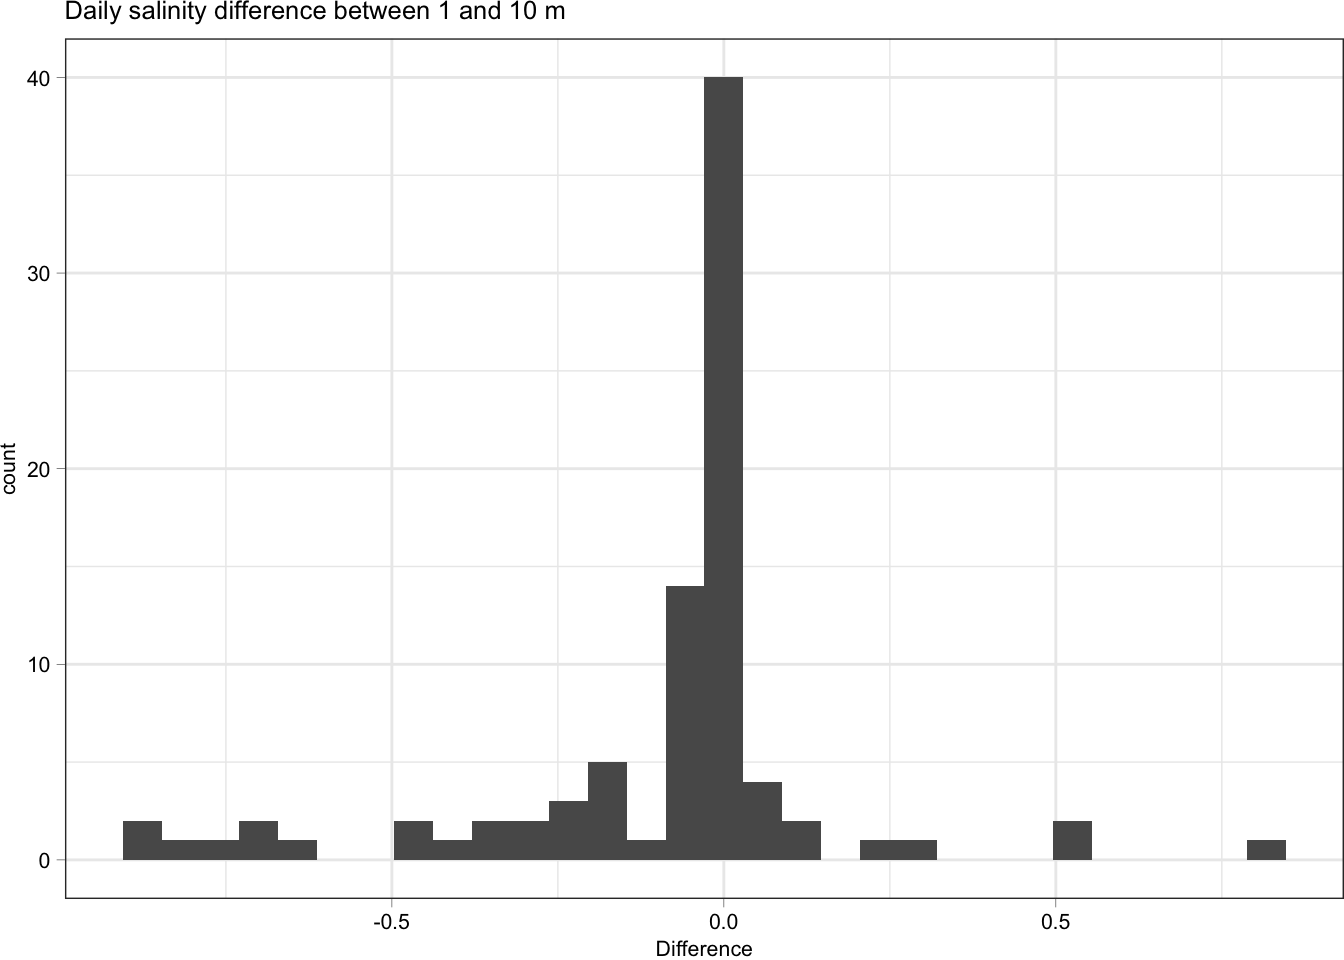
\includegraphics[width=0.8\linewidth]{awipev-CO2_files/figure-latex/Sal profile-2}
There are 184 days with salinity values at both 1 m (0-2 m) and 9 m
(\textgreater{} 8 m). The salinity difference between 1 and 9 m ranges
between -4.404125 and 2.1417658 (mean: -0.3428293; -0.0681155). The
difference with depth is therefore significant.

\hypertarget{sal-fb-sal-ctd-9-m}{%
\subsubsection{\texorpdfstring{\textbf{Sal FB / Sal CTD 9 m
}}{Sal FB / Sal CTD 9 m }}\label{sal-fb-sal-ctd-9-m}}

\begin{center}\includegraphics[width=0.8\linewidth]{awipev-CO2_files/figure-latex/Sal comparaison-1} \end{center}

The mean difference between salinity FB and in situ is: -0.16 ± 0.88
PSU.

\hypertarget{temperatures}{%
\subsection{Temperatures}\label{temperatures}}

Several temperature sensors are on site, 1 inside the Ferrybox (SBE45),
5 outside (ctd183, ctd181, ctd578, ctd964/964b and ctd103) that are
switched periodically and 1 fixed at 11 m depth (sbe38). Temperature in
situ at 11 m depth is taken in consideration. If data gaps are
encountered, they are filled with bottom temperature data from ctd
(\textgreater{} 8 m). New column ``temp\_mix'' is created. For the
moment, no gaps are encountered and temp\_mix = temp\_insitu\_11m.

\begin{itemize}
\tightlist
\item
  1 SBE45 inside the Ferrybox (temp\_fb)
\item
  5 CTD profiling (temp\_insitu\_ctd\_1m - 3m - 5m - 7m - 9m)
\item
  1 fixed at 11 meters depth (temp\_insitu\_11m)
\end{itemize}

\textbackslash begin\{center\}\includegraphics[width=0.8\linewidth]{awipev-CO2_files/figure-latex/temperature time series-1}
\includegraphics[width=0.8\linewidth]{awipev-CO2_files/figure-latex/temperature time series-2}

\hypertarget{temperature-profiles}{%
\subsubsection{\texorpdfstring{\textbf{Temperature
profiles}}{Temperature profiles}}\label{temperature-profiles}}

\textbackslash begin\{center\}\includegraphics[width=0.8\linewidth]{awipev-CO2_files/figure-latex/temperature profiles-1}
There are 184 days with temperature values at both 1 m (0-2 m) and 9 m
(\textgreater{} 8 m). The temperature difference between 1 and 9 m
ranges between -4.0276557°C and 1.8536989°C (mean: -0.2577894°C;
-0.1372184°C). The difference with depth is therefore significant.

\hypertarget{t-ferrybox-t-insitu-11-m}{%
\subsubsection{\texorpdfstring{\textbf{T Ferrybox / T insitu 11 m
}}{T Ferrybox / T insitu 11 m }}\label{t-ferrybox-t-insitu-11-m}}

\includegraphics{awipev-CO2_files/figure-latex/Temp fb insi comparaison-1.pdf}

The mean difference between temperature Ferrybox and in situ at 11 m is:
0.53 ± 0.2°C.

\hypertarget{t-11-m-t-ctd-8-m}{%
\subsubsection{\texorpdfstring{\textbf{T 11 m / T CTD \textgreater{} 8 m
}}{T 11 m / T CTD \textgreater{} 8 m }}\label{t-11-m-t-ctd-8-m}}

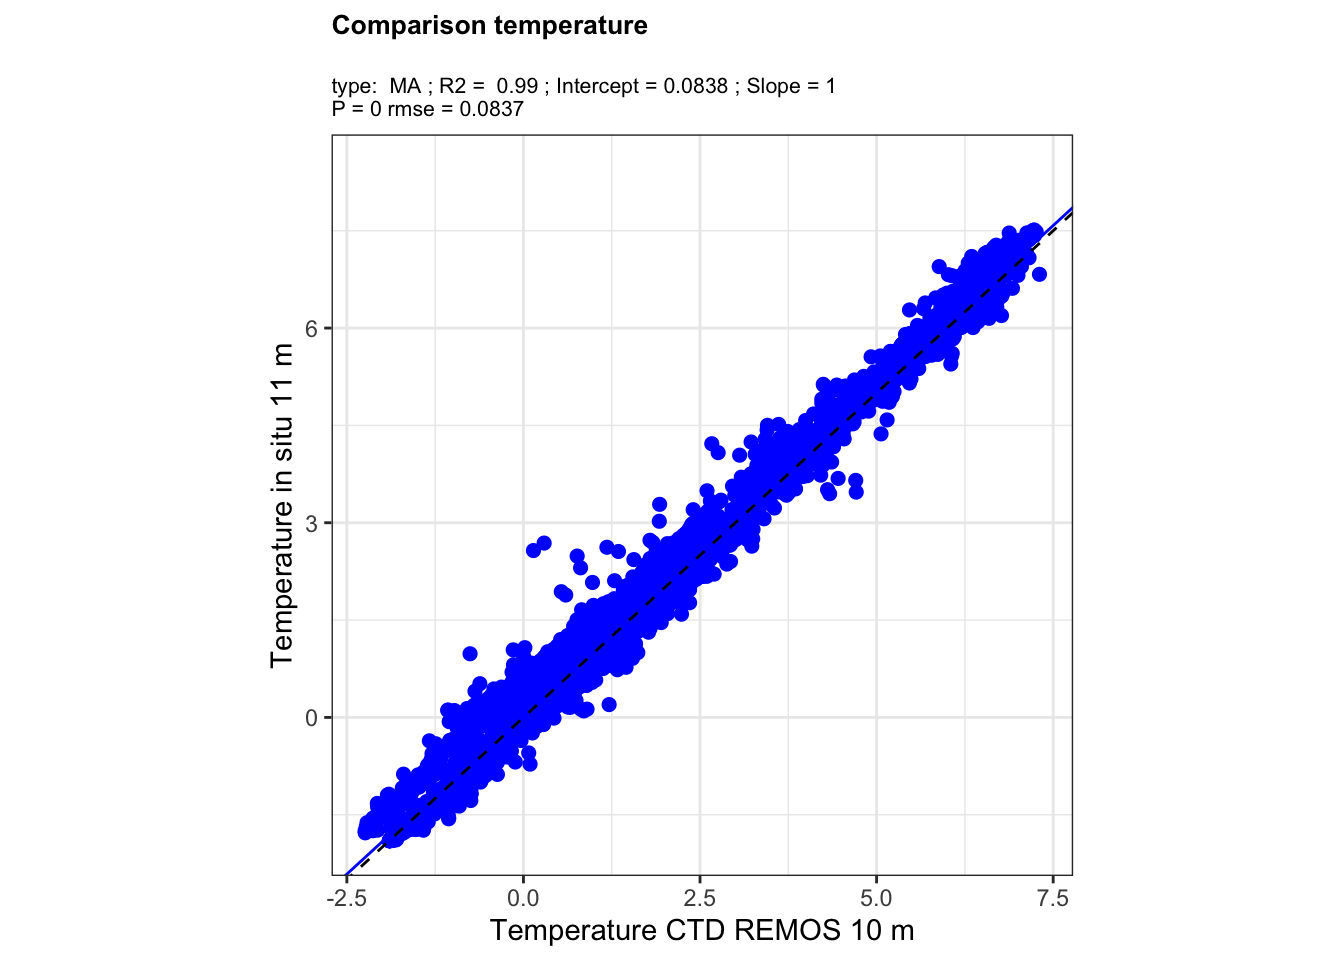
\includegraphics{awipev-CO2_files/figure-latex/Temp 11m and ctd comparaison-1.pdf}

The mean difference between temperature Ferrybox and in situ at 11 m is:
-0.04 ± 0.34°C.

\hypertarget{total-alkalinity}{%
\subsection{Total alkalinity}\label{total-alkalinity}}

Since we bought the AT analyser (February 2016), numerous problems
happened due to a leak of the degassing unit in each analyser and sudden
step changes. Last analyser repaired by Contros was installed back in
the FB on 2018-07-31. This was the 3rd analyser on site. Even with this
instrument, data collection didn't show satisfaction.

\hypertarget{discrete-total-alkalinity-reference-vs-salinity-relationship}{%
\subsubsection{\texorpdfstring{\textbf{Discrete total alkalinity
(reference) vs salinity
relationship}}{Discrete total alkalinity (reference) vs salinity relationship}}\label{discrete-total-alkalinity-reference-vs-salinity-relationship}}

In the previous part, missing TA were interpolated with a linear model.
This does not reflect the natural variability of TA. For this reason,
missing TA is now calculated from salinity data by making a relationship
between the same reference TA samples as in the previous part and
salinity data.

The relationship between titrated total alkalinity (references) and
salinity is very good with an r2 of . Need to compare with other
relationships from the literature.

\begin{center}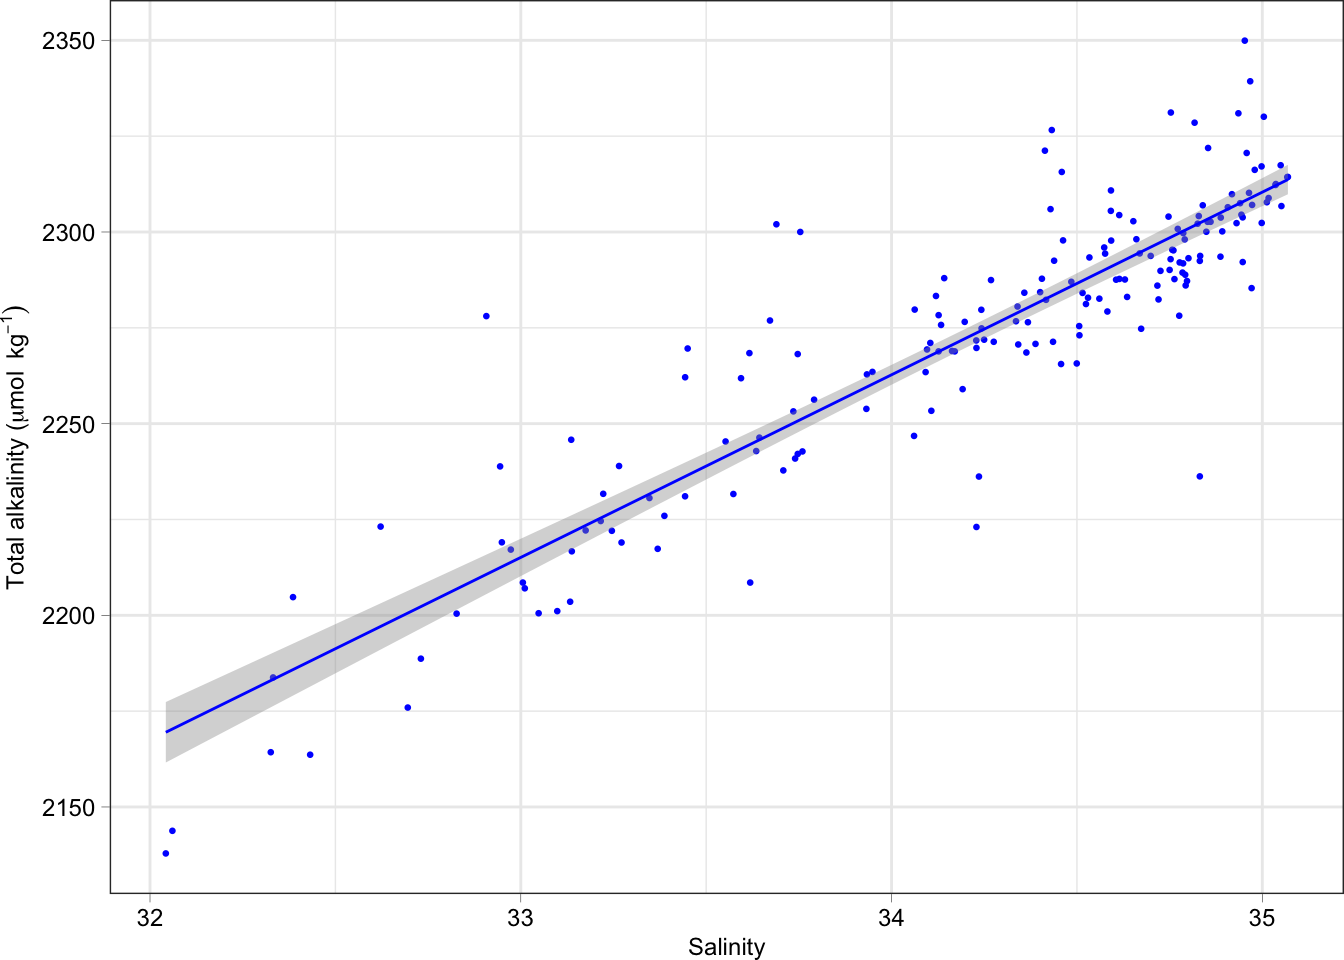
\includegraphics[width=1\linewidth]{awipev-CO2_files/figure-latex/plot Discrete salinity vs TA-1} \end{center}

\hypertarget{final-ta-re-calculated-data-salinity-relationship}{%
\paragraph{\texorpdfstring{\textbf{Final TA re-calculated data (Salinity
relationship)}}{Final TA re-calculated data (Salinity relationship)}}\label{final-ta-re-calculated-data-salinity-relationship}}

\includegraphics[width=1\linewidth]{awipev-CO2_files/figure-latex/Plot TA calc TA meas-1}

There are a lot of outliers in the 4th period (since the new analyzer
was set up in Nov.~2018). We use the desplike function to remove them.

\hypertarget{pco2}{%
\subsection{\texorpdfstring{\emph{p}CO\textsubscript{2}}{pCO2}}\label{pco2}}

The HydroC CO\textsubscript{2} FT sensor (S/N: CO2FT-0215-001) was
bought from Contros (Germany) in February 2015. It was deployed in the
FerryBox with other sensors since July 2015, the 20th. A spare sensor
(S/N: CO2FT-0515-001) was also bought in March 2015 and carried to
Ny-Alesund to replace the first one in case of calibration or problem.
Both sensors were set on a cycle according to informations given by
Contros in March 2015
(\href{mailto:c.kirbach@contros.eu}{\nolinkurl{c.kirbach@contros.eu}}):

30 min warm up --\textgreater{} (3 min Zeroing + 15 min Flushing + 702
minutes Measuring) --\textgreater{} (3 + 15 + 702)\ldots{}

\begin{itemize}
\tightlist
\item
  \textbf{Warm-up}: running without sending data. Done once, after the
  sensor is turned on. Time can vary depending on T water and power
  supply.
\item
  \textbf{Flushing}: running normally. Phase of equilibration that
  depends on the sensor configuration and the environment conditions.
  Warmer the water is and larger the flow is in front of the membrane,
  faster will be the response time and shorter will be the flush time.
  Recovery data of the sensor signal from the zeroing interval happen in
  this time. During this step the flush flag is set to ``1'' for
  simplifier extraction of the flush values.
\item
  \textbf{Measuring}: running normally and all other flags are on ``0''.
  Sensor is fully equilibrated and T is stable.
\end{itemize}

During those steps (except zeroing) the sensor runs normally.
Equilibration between the gas inside the sensor and the dissolved gas in
ambient water takes place. Gas is led to NDIR unit while T control is
running.

\hypertarget{corrected-contros-vs-calculated-pco2-data}{%
\subsubsection{\texorpdfstring{\textbf{Corrected Contros vs calculated
\emph{p}CO\textsubscript{2}
data}}{Corrected Contros vs calculated pCO2 data}}\label{corrected-contros-vs-calculated-pco2-data}}

The relationship between the Contros and calculated
\emph{p}CO\textsubscript{2} is not good at all in the sense that it is
far from the 1:1 line, despite a good r2 (0.65).

\begin{center}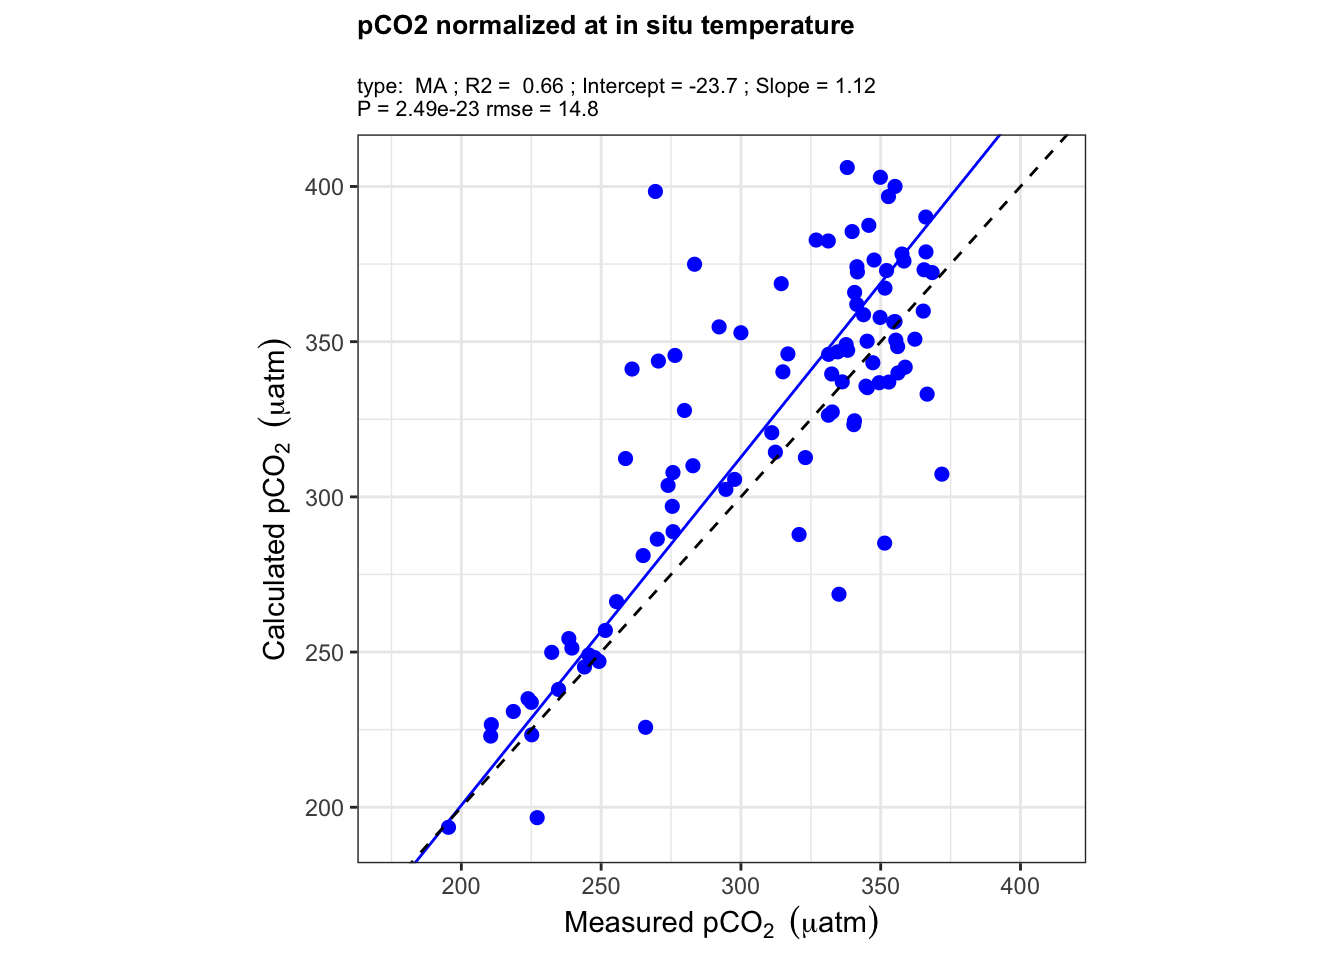
\includegraphics[width=1\linewidth]{awipev-CO2_files/figure-latex/plot measured vs calculated pCO2-1} \end{center}

\hypertarget{final-pco2-data}{%
\subsubsection{\texorpdfstring{\textbf{Final \emph{p}CO\textsubscript{2}
data}}{Final pCO2 data}}\label{final-pco2-data}}

\begin{center}\includegraphics[width=1\linewidth]{awipev-CO2_files/figure-latex/Final pCO2-1} \end{center}

\hypertarget{ph-seafet}{%
\subsection{pH seaFET}\label{ph-seafet}}

pH is measured continuously by an autonomous seaFET pH sensor. Because
of issue, measurement periodicity was set to 1 hour from 2018-02-02 to
2018-04-17. \emph{Note that the pH sensor is mounted on a profiling
structure. Here, only seaFET data recorded with a depth \textgreater{} 8
m are taken in consideration.} pH calibration is based on monthly
discrete samples that are analysed with spectrophotometric method in
Villefranche by Samir Alliouane. When it is not possible to sample at
the vicinity of the sensor for practice reasons (in winter), sampling is
done in the harbour and is not taken in consideration for calibration
for spatial reasons.

Calibration was done following the methods and code described in
Bresnahan et al.~(2014) and adapted to use in R (seacarb package).
Deployment periods are difined so that one spectrophotometric
measurement is in the middle of a defined period of calibration (shaded
colors in the plot).

Within this deployment period, calibration is made with E0 calculation
(first plot) and final corrected pH is calculated (second plot). To
allow calibration, one spectrophotometric pH measurement must match:
seaFET voltage, in situ temperature (SBE38) and salinity. When one of
these parameters is missing for any reasons (Ferrybox maintenance,
breakdown\ldots), the gap is filled with a mean of the 4 previous or
next hours when available. If the pH spectrophotometric measurement is
too far from the available values, the calibration is not performed
(environemental variability reasons). The SBE38 insitu temperature and
seaFET temperature are very similar (slope = 0.992, r2 = 0.96, see tab
``Temperatures''). These two temperatures were used interchangeably if
one is missing.

Missing data which could be estimated on : 2017-08-24, 2017-09-28,
2019-09-13 x 2. Missing data which could not be estimated on :
2018-04-16 , 2018-12-14, 2019-01-18.

We decided to change the calculation of E0. Before E0 was calculated for
each pH spectro measurements. Now, EO is calculated making a mean of
several E0 that come from one deployment period (sensor in the water for
several months).

\hypertarget{seafet-calibration-constant-e0}{%
\subsubsection{\texorpdfstring{\textbf{seaFET calibration constant
E0}}{seaFET calibration constant E0}}\label{seafet-calibration-constant-e0}}

Plots of E0int25 and E0ext25 returned by the function ``pHCalib'' for
each period of deployement are shown below.

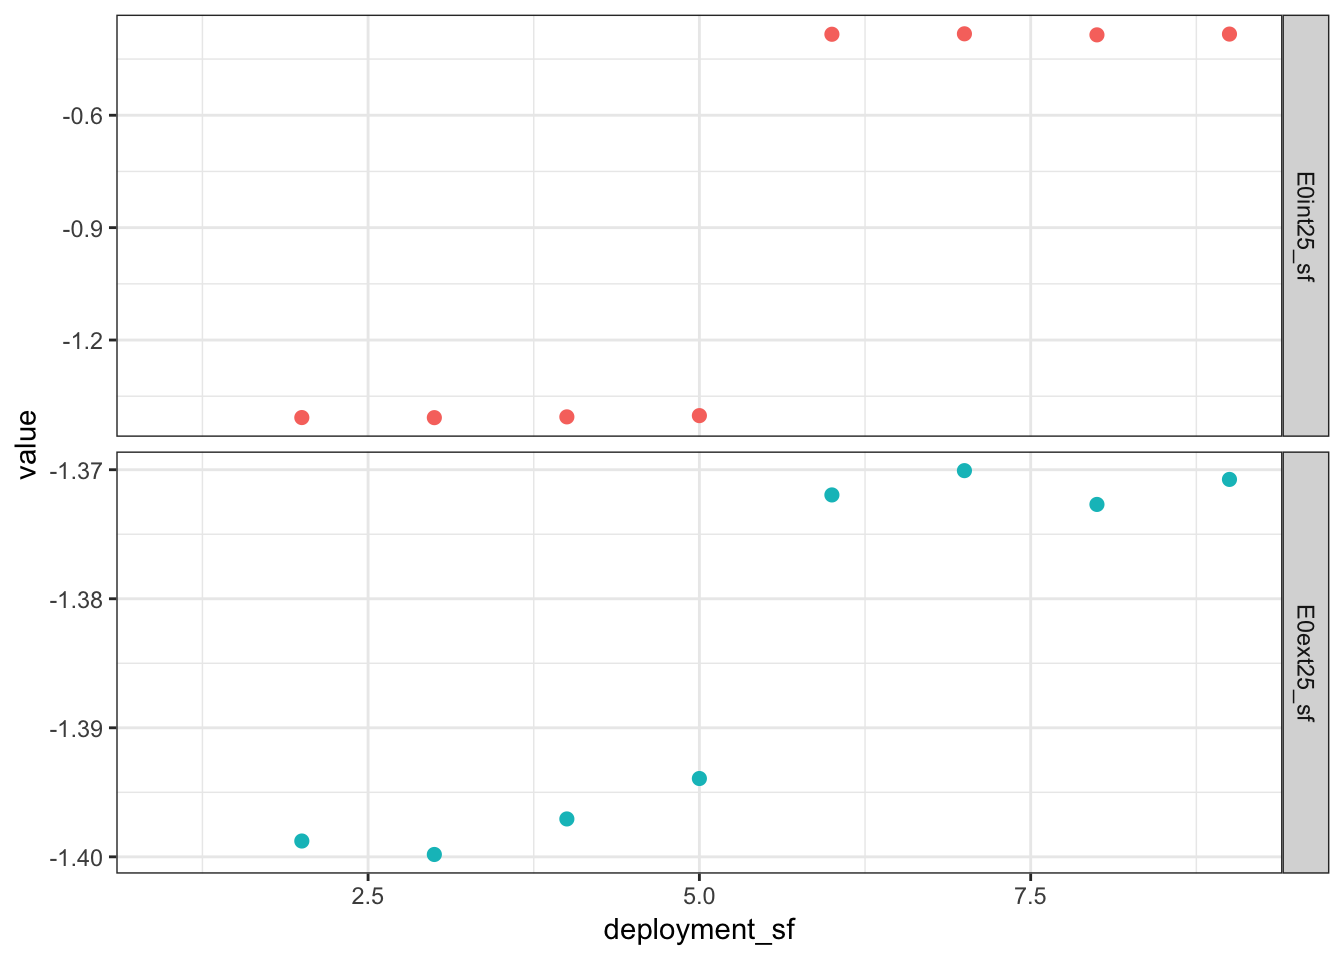
\includegraphics[width=0.6\linewidth]{awipev-CO2_files/figure-latex/seaFET calibration sf_calib-1}

\hypertarget{seafet-pht-calibrated}{%
\subsubsection{\texorpdfstring{\textbf{seaFET pHT
calibrated}}{seaFET pHT calibrated}}\label{seafet-pht-calibrated}}

pH is measured continuously by an autonomous seaFET pH sensor. Final
calibrated seaFET pHT data (green dots) are shown here after calibration
with spectro measurements (red dots) according to each period of
deployement, defined between 2 spectro measurements (shading grey).
Calibration was done following the methods and code described in
Bresnahan \emph{et al.} (2014) using seaFET voltage and spectro
measurements. During the fifth period, seaFET cannot be calibrated
because seaFET was not working during the time of reference (pH spectro)
sampling (2018-04-16). To solve this calibration, we decided to fit the
spectro measurement with a pH mean of 4 previous days.

We also defined a period of malfunction from \textbf{2017-12-14} to
\textbf{2018-02-02}. in the first part of this period, until 2018-01-08,
we decided to filter outliers. In the second part, until the end of the
period, data must be removed.

\includegraphics{awipev-CO2_files/figure-latex/seaFET pH calculation sf_calc-1.pdf}

\hypertarget{seafet-ph-profiles}{%
\subsubsection{\texorpdfstring{\textbf{seaFET pH
profiles}}{seaFET pH profiles}}\label{seafet-ph-profiles}}

\begin{verbatim}
##                        Df Sum Sq Mean Sq F value Pr(>F)    
## tmp$depth               1  0.478  0.4784   182.7 <2e-16 ***
## tmp$montht             11 12.237  1.1125   424.8 <2e-16 ***
## tmp$depth:tmp$montht   11  5.667  0.5152   196.7 <2e-16 ***
## Residuals            8773 22.976  0.0026                   
## ---
## Signif. codes:  0 '***' 0.001 '**' 0.01 '*' 0.05 '.' 0.1 ' ' 1
## 8753 observations deleted due to missingness
\end{verbatim}

\begin{center}\includegraphics[width=0.8\linewidth]{awipev-CO2_files/figure-latex/seafet profile-1} \includegraphics[width=0.8\linewidth]{awipev-CO2_files/figure-latex/seafet profile-2} \end{center}

\textbf{Conclusion}: The range is significantly larger during some
months when the data deeper than 8 m are considered. Also, pH is
sometimes higher at the surface, at other times it is higher on the
bottom (June). No data are available at 1 m (actually 0 to 2 m). So, to
compare surface and bottom, I combine 1 and 3 m (0 to 4 m) and 9 m
(below 8 m).

Depth and month of the year have a statistically significant effet on
pH. The interaxction is also significant, indicating that the effect of
depth differs depending on the month.

\begin{itemize}
\tightlist
\item
  To compare with pCO2/pCO2 measured in the Ferrybox seems therefore
  better to stick with pH\_9m, that is at depths deeper than 8 m.
\item
  pCO2 would have the same behaviour as pH. For air-sea CO2 fluxes, one
  should use data from 0 to 4 m.
\end{itemize}

\hypertarget{ph-durafet}{%
\subsection{pH durafet}\label{ph-durafet}}

pH is measured continuously by an autonomous durafet pH sensor. Final
calibrated durafet pHT data (green dots) are shown here after
calibration with spectro measurements (red dots) according to each
period of deployement, defined between 2 spectro measurements (shading
grey). Calibration was done appliying an offset of pH between measured
and spectro data per periods.

\hypertarget{durafet-calibration}{%
\subsubsection{\texorpdfstring{\textbf{Durafet
calibration}}{Durafet calibration}}\label{durafet-calibration}}

\includegraphics{awipev-CO2_files/figure-latex/durafet calibration-1.pdf}
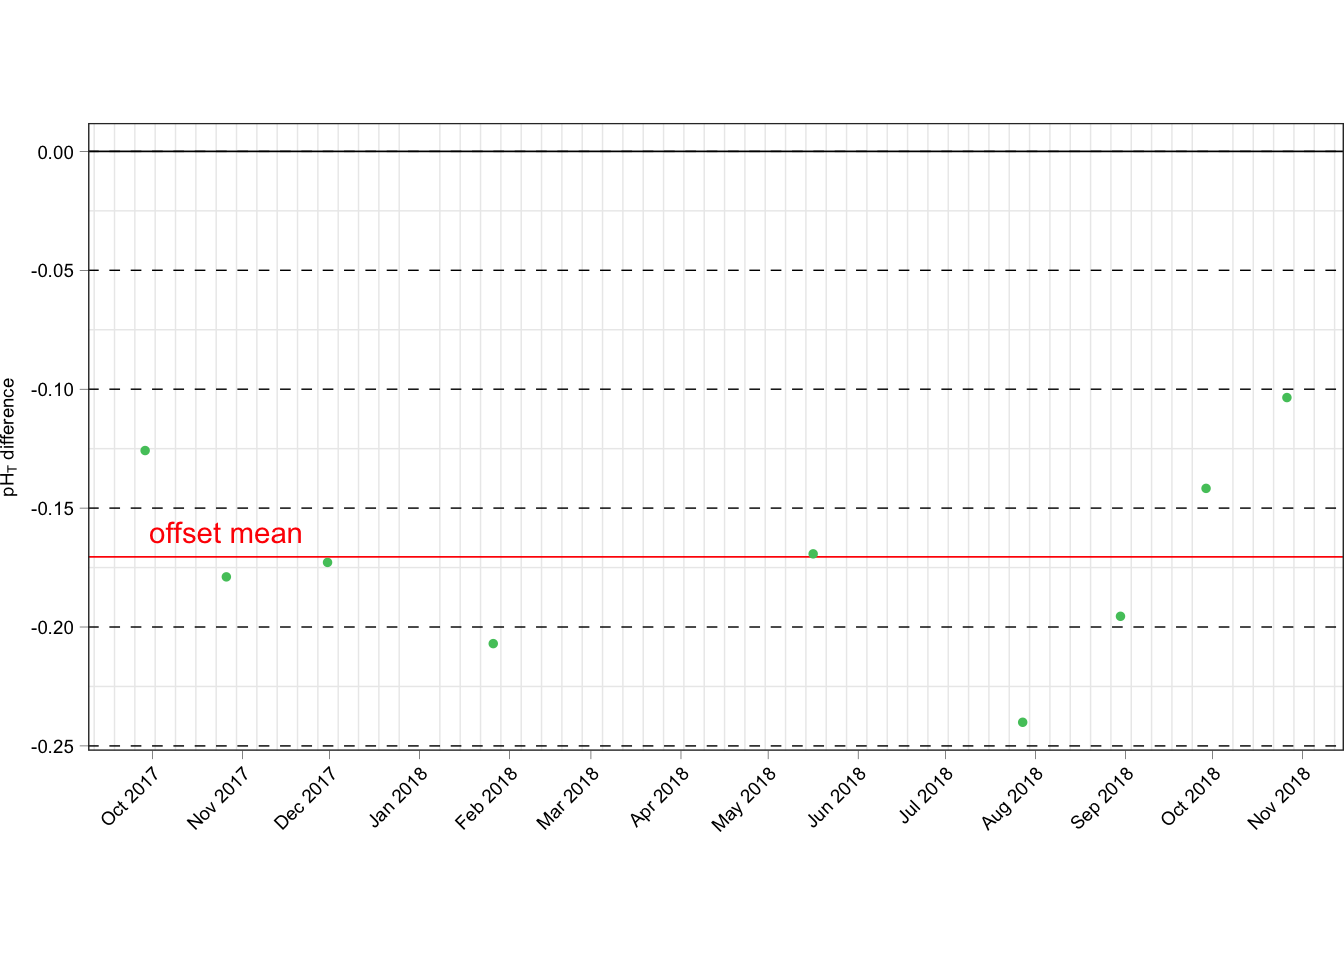
\includegraphics{awipev-CO2_files/figure-latex/durafet calibration-2.pdf}
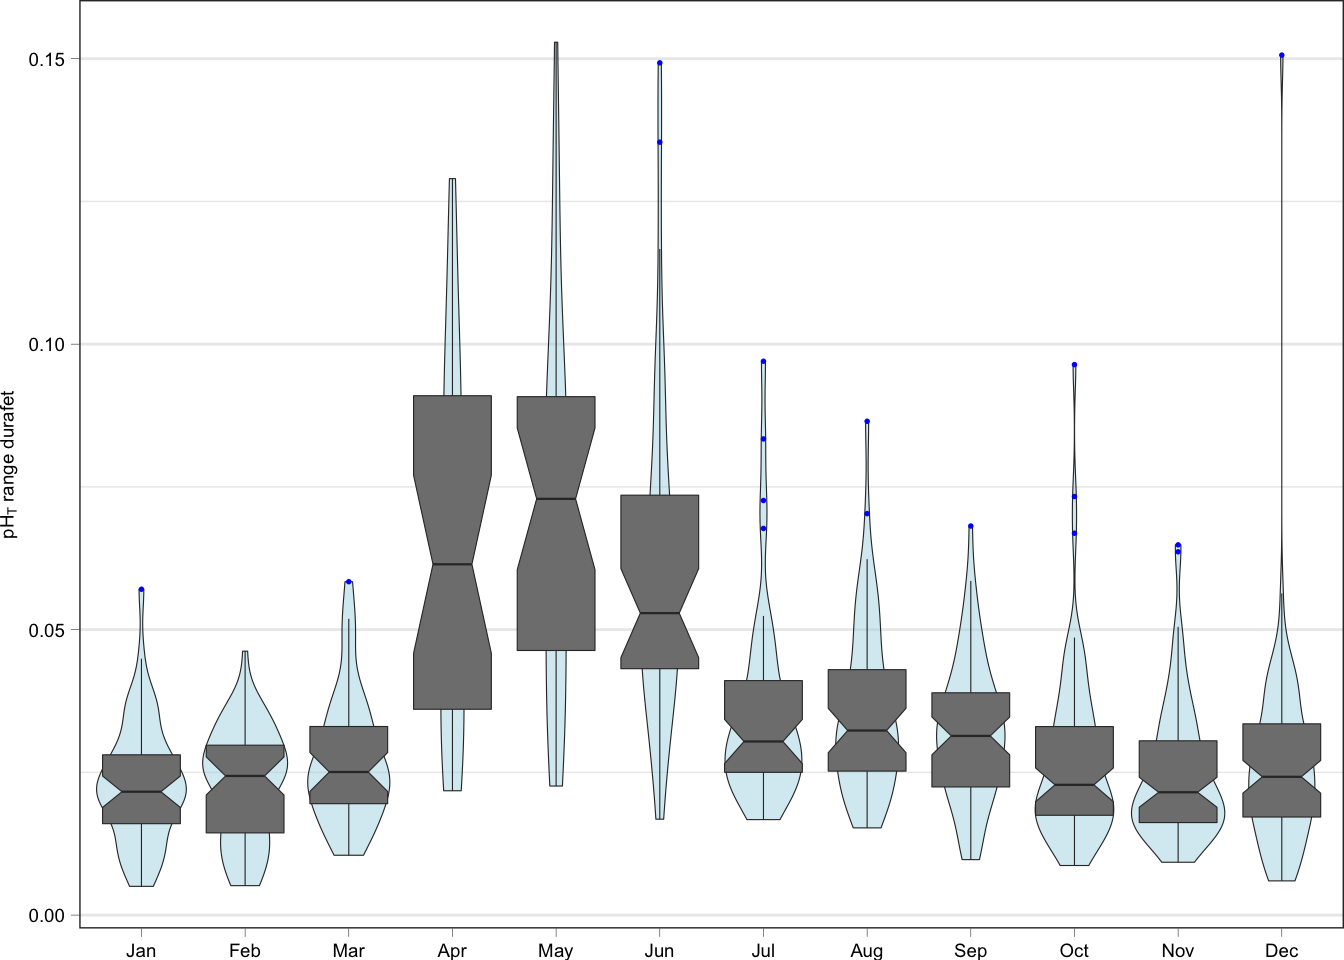
\includegraphics{awipev-CO2_files/figure-latex/durafet calibration-3.pdf}

The average offset between durafet and references (spectro) data is
-0.16 pH unit (sd = 0.04, n = 25).

\hypertarget{range-per-months}{%
\subsection{Range per months}\label{range-per-months}}

\begin{longtable}[]{@{}lrrrrrrrrrrrrrrrrrrrrrrrrrrrrrrrr@{}}
\toprule
\begin{minipage}[b]{(\columnwidth - 32\tabcolsep) * \real{0.02}}\raggedright
montht\strut
\end{minipage} &
\begin{minipage}[b]{(\columnwidth - 32\tabcolsep) * \real{0.03}}\raggedleft
temp\_mix\_max\strut
\end{minipage} &
\begin{minipage}[b]{(\columnwidth - 32\tabcolsep) * \real{0.03}}\raggedleft
temp\_mix\_min\strut
\end{minipage} &
\begin{minipage}[b]{(\columnwidth - 32\tabcolsep) * \real{0.03}}\raggedleft
temp\_ctd\_1m\_max\strut
\end{minipage} &
\begin{minipage}[b]{(\columnwidth - 32\tabcolsep) * \real{0.03}}\raggedleft
temp\_ctd\_1m\_min\strut
\end{minipage} &
\begin{minipage}[b]{(\columnwidth - 32\tabcolsep) * \real{0.03}}\raggedleft
temp\_ctd\_3m\_max\strut
\end{minipage} &
\begin{minipage}[b]{(\columnwidth - 32\tabcolsep) * \real{0.03}}\raggedleft
temp\_ctd\_3m\_min\strut
\end{minipage} &
\begin{minipage}[b]{(\columnwidth - 32\tabcolsep) * \real{0.03}}\raggedleft
temp\_ctd\_5m\_max\strut
\end{minipage} &
\begin{minipage}[b]{(\columnwidth - 32\tabcolsep) * \real{0.03}}\raggedleft
temp\_ctd\_5m\_min\strut
\end{minipage} &
\begin{minipage}[b]{(\columnwidth - 32\tabcolsep) * \real{0.03}}\raggedleft
temp\_ctd\_7m\_max\strut
\end{minipage} &
\begin{minipage}[b]{(\columnwidth - 32\tabcolsep) * \real{0.03}}\raggedleft
temp\_ctd\_7m\_min\strut
\end{minipage} &
\begin{minipage}[b]{(\columnwidth - 32\tabcolsep) * \real{0.03}}\raggedleft
temp\_ctd\_9m\_max\strut
\end{minipage} &
\begin{minipage}[b]{(\columnwidth - 32\tabcolsep) * \real{0.03}}\raggedleft
temp\_ctd\_9m\_min\strut
\end{minipage} &
\begin{minipage}[b]{(\columnwidth - 32\tabcolsep) * \real{0.03}}\raggedleft
temp\_11m\_max\strut
\end{minipage} &
\begin{minipage}[b]{(\columnwidth - 32\tabcolsep) * \real{0.03}}\raggedleft
temp\_11m\_min\strut
\end{minipage} &
\begin{minipage}[b]{(\columnwidth - 32\tabcolsep) * \real{0.03}}\raggedleft
temp\_fb\_max\strut
\end{minipage} &
\begin{minipage}[b]{(\columnwidth - 32\tabcolsep) * \real{0.03}}\raggedleft
temp\_fb\_min\strut
\end{minipage} &
\begin{minipage}[b]{(\columnwidth - 32\tabcolsep) * \real{0.03}}\raggedleft
sal\_mix\_max\strut
\end{minipage} &
\begin{minipage}[b]{(\columnwidth - 32\tabcolsep) * \real{0.03}}\raggedleft
sal\_mix\_min\strut
\end{minipage} &
\begin{minipage}[b]{(\columnwidth - 32\tabcolsep) * \real{0.03}}\raggedleft
sal\_ctd\_1m\_max\strut
\end{minipage} &
\begin{minipage}[b]{(\columnwidth - 32\tabcolsep) * \real{0.03}}\raggedleft
sal\_ctd\_1m\_min\strut
\end{minipage} &
\begin{minipage}[b]{(\columnwidth - 32\tabcolsep) * \real{0.03}}\raggedleft
sal\_ctd\_3m\_max\strut
\end{minipage} &
\begin{minipage}[b]{(\columnwidth - 32\tabcolsep) * \real{0.03}}\raggedleft
sal\_ctd\_3m\_min\strut
\end{minipage} &
\begin{minipage}[b]{(\columnwidth - 32\tabcolsep) * \real{0.03}}\raggedleft
sal\_ctd\_5m\_max\strut
\end{minipage} &
\begin{minipage}[b]{(\columnwidth - 32\tabcolsep) * \real{0.03}}\raggedleft
sal\_ctd\_5m\_min\strut
\end{minipage} &
\begin{minipage}[b]{(\columnwidth - 32\tabcolsep) * \real{0.03}}\raggedleft
sal\_ctd\_7m\_max\strut
\end{minipage} &
\begin{minipage}[b]{(\columnwidth - 32\tabcolsep) * \real{0.03}}\raggedleft
sal\_ctd\_7m\_min\strut
\end{minipage} &
\begin{minipage}[b]{(\columnwidth - 32\tabcolsep) * \real{0.03}}\raggedleft
sal\_ctd\_9m\_max\strut
\end{minipage} &
\begin{minipage}[b]{(\columnwidth - 32\tabcolsep) * \real{0.03}}\raggedleft
sal\_ctd\_9m\_min\strut
\end{minipage} &
\begin{minipage}[b]{(\columnwidth - 32\tabcolsep) * \real{0.02}}\raggedleft
sal\_fb\_max\strut
\end{minipage} &
\begin{minipage}[b]{(\columnwidth - 32\tabcolsep) * \real{0.02}}\raggedleft
sal\_fb\_min\strut
\end{minipage} &
\begin{minipage}[b]{(\columnwidth - 32\tabcolsep) * \real{0.02}}\raggedleft
pH\_sf\_max\strut
\end{minipage} &
\begin{minipage}[b]{(\columnwidth - 32\tabcolsep) * \real{0.02}}\raggedleft
pH\_sf\_min\strut
\end{minipage}\tabularnewline
\midrule
\endhead
\begin{minipage}[t]{(\columnwidth - 32\tabcolsep) * \real{0.02}}\raggedright
Jan\strut
\end{minipage} &
\begin{minipage}[t]{(\columnwidth - 32\tabcolsep) * \real{0.03}}\raggedleft
4.03\strut
\end{minipage} &
\begin{minipage}[t]{(\columnwidth - 32\tabcolsep) * \real{0.03}}\raggedleft
-1.90\strut
\end{minipage} &
\begin{minipage}[t]{(\columnwidth - 32\tabcolsep) * \real{0.03}}\raggedleft
3.84\strut
\end{minipage} &
\begin{minipage}[t]{(\columnwidth - 32\tabcolsep) * \real{0.03}}\raggedleft
-1.49\strut
\end{minipage} &
\begin{minipage}[t]{(\columnwidth - 32\tabcolsep) * \real{0.03}}\raggedleft
3.86\strut
\end{minipage} &
\begin{minipage}[t]{(\columnwidth - 32\tabcolsep) * \real{0.03}}\raggedleft
-1.88\strut
\end{minipage} &
\begin{minipage}[t]{(\columnwidth - 32\tabcolsep) * \real{0.03}}\raggedleft
3.78\strut
\end{minipage} &
\begin{minipage}[t]{(\columnwidth - 32\tabcolsep) * \real{0.03}}\raggedleft
-1.86\strut
\end{minipage} &
\begin{minipage}[t]{(\columnwidth - 32\tabcolsep) * \real{0.03}}\raggedleft
3.92\strut
\end{minipage} &
\begin{minipage}[t]{(\columnwidth - 32\tabcolsep) * \real{0.03}}\raggedleft
-1.86\strut
\end{minipage} &
\begin{minipage}[t]{(\columnwidth - 32\tabcolsep) * \real{0.03}}\raggedleft
4.04\strut
\end{minipage} &
\begin{minipage}[t]{(\columnwidth - 32\tabcolsep) * \real{0.03}}\raggedleft
-1.83\strut
\end{minipage} &
\begin{minipage}[t]{(\columnwidth - 32\tabcolsep) * \real{0.03}}\raggedleft
4.03\strut
\end{minipage} &
\begin{minipage}[t]{(\columnwidth - 32\tabcolsep) * \real{0.03}}\raggedleft
-1.90\strut
\end{minipage} &
\begin{minipage}[t]{(\columnwidth - 32\tabcolsep) * \real{0.03}}\raggedleft
4.27\strut
\end{minipage} &
\begin{minipage}[t]{(\columnwidth - 32\tabcolsep) * \real{0.03}}\raggedleft
-1.25\strut
\end{minipage} &
\begin{minipage}[t]{(\columnwidth - 32\tabcolsep) * \real{0.03}}\raggedleft
34.91\strut
\end{minipage} &
\begin{minipage}[t]{(\columnwidth - 32\tabcolsep) * \real{0.03}}\raggedleft
33.84\strut
\end{minipage} &
\begin{minipage}[t]{(\columnwidth - 32\tabcolsep) * \real{0.03}}\raggedleft
35.37\strut
\end{minipage} &
\begin{minipage}[t]{(\columnwidth - 32\tabcolsep) * \real{0.03}}\raggedleft
29.15\strut
\end{minipage} &
\begin{minipage}[t]{(\columnwidth - 32\tabcolsep) * \real{0.03}}\raggedleft
35.37\strut
\end{minipage} &
\begin{minipage}[t]{(\columnwidth - 32\tabcolsep) * \real{0.03}}\raggedleft
28.56\strut
\end{minipage} &
\begin{minipage}[t]{(\columnwidth - 32\tabcolsep) * \real{0.03}}\raggedleft
35.35\strut
\end{minipage} &
\begin{minipage}[t]{(\columnwidth - 32\tabcolsep) * \real{0.03}}\raggedleft
29.16\strut
\end{minipage} &
\begin{minipage}[t]{(\columnwidth - 32\tabcolsep) * \real{0.03}}\raggedleft
35.35\strut
\end{minipage} &
\begin{minipage}[t]{(\columnwidth - 32\tabcolsep) * \real{0.03}}\raggedleft
28.00\strut
\end{minipage} &
\begin{minipage}[t]{(\columnwidth - 32\tabcolsep) * \real{0.03}}\raggedleft
35.37\strut
\end{minipage} &
\begin{minipage}[t]{(\columnwidth - 32\tabcolsep) * \real{0.03}}\raggedleft
28.01\strut
\end{minipage} &
\begin{minipage}[t]{(\columnwidth - 32\tabcolsep) * \real{0.02}}\raggedleft
34.91\strut
\end{minipage} &
\begin{minipage}[t]{(\columnwidth - 32\tabcolsep) * \real{0.02}}\raggedleft
34.06\strut
\end{minipage} &
\begin{minipage}[t]{(\columnwidth - 32\tabcolsep) * \real{0.02}}\raggedleft
8.0925\strut
\end{minipage} &
\begin{minipage}[t]{(\columnwidth - 32\tabcolsep) * \real{0.02}}\raggedleft
7.9461\strut
\end{minipage}\tabularnewline
\begin{minipage}[t]{(\columnwidth - 32\tabcolsep) * \real{0.02}}\raggedright
Feb\strut
\end{minipage} &
\begin{minipage}[t]{(\columnwidth - 32\tabcolsep) * \real{0.03}}\raggedleft
2.80\strut
\end{minipage} &
\begin{minipage}[t]{(\columnwidth - 32\tabcolsep) * \real{0.03}}\raggedleft
-1.91\strut
\end{minipage} &
\begin{minipage}[t]{(\columnwidth - 32\tabcolsep) * \real{0.03}}\raggedleft
1.90\strut
\end{minipage} &
\begin{minipage}[t]{(\columnwidth - 32\tabcolsep) * \real{0.03}}\raggedleft
-2.24\strut
\end{minipage} &
\begin{minipage}[t]{(\columnwidth - 32\tabcolsep) * \real{0.03}}\raggedleft
2.36\strut
\end{minipage} &
\begin{minipage}[t]{(\columnwidth - 32\tabcolsep) * \real{0.03}}\raggedleft
-2.24\strut
\end{minipage} &
\begin{minipage}[t]{(\columnwidth - 32\tabcolsep) * \real{0.03}}\raggedleft
2.32\strut
\end{minipage} &
\begin{minipage}[t]{(\columnwidth - 32\tabcolsep) * \real{0.03}}\raggedleft
-2.24\strut
\end{minipage} &
\begin{minipage}[t]{(\columnwidth - 32\tabcolsep) * \real{0.03}}\raggedleft
2.69\strut
\end{minipage} &
\begin{minipage}[t]{(\columnwidth - 32\tabcolsep) * \real{0.03}}\raggedleft
-2.24\strut
\end{minipage} &
\begin{minipage}[t]{(\columnwidth - 32\tabcolsep) * \real{0.03}}\raggedleft
2.86\strut
\end{minipage} &
\begin{minipage}[t]{(\columnwidth - 32\tabcolsep) * \real{0.03}}\raggedleft
-1.96\strut
\end{minipage} &
\begin{minipage}[t]{(\columnwidth - 32\tabcolsep) * \real{0.03}}\raggedleft
2.80\strut
\end{minipage} &
\begin{minipage}[t]{(\columnwidth - 32\tabcolsep) * \real{0.03}}\raggedleft
-1.91\strut
\end{minipage} &
\begin{minipage}[t]{(\columnwidth - 32\tabcolsep) * \real{0.03}}\raggedleft
3.02\strut
\end{minipage} &
\begin{minipage}[t]{(\columnwidth - 32\tabcolsep) * \real{0.03}}\raggedleft
-1.35\strut
\end{minipage} &
\begin{minipage}[t]{(\columnwidth - 32\tabcolsep) * \real{0.03}}\raggedleft
34.97\strut
\end{minipage} &
\begin{minipage}[t]{(\columnwidth - 32\tabcolsep) * \real{0.03}}\raggedleft
34.21\strut
\end{minipage} &
\begin{minipage}[t]{(\columnwidth - 32\tabcolsep) * \real{0.03}}\raggedleft
35.10\strut
\end{minipage} &
\begin{minipage}[t]{(\columnwidth - 32\tabcolsep) * \real{0.03}}\raggedleft
34.44\strut
\end{minipage} &
\begin{minipage}[t]{(\columnwidth - 32\tabcolsep) * \real{0.03}}\raggedleft
35.11\strut
\end{minipage} &
\begin{minipage}[t]{(\columnwidth - 32\tabcolsep) * \real{0.03}}\raggedleft
32.62\strut
\end{minipage} &
\begin{minipage}[t]{(\columnwidth - 32\tabcolsep) * \real{0.03}}\raggedleft
35.11\strut
\end{minipage} &
\begin{minipage}[t]{(\columnwidth - 32\tabcolsep) * \real{0.03}}\raggedleft
31.21\strut
\end{minipage} &
\begin{minipage}[t]{(\columnwidth - 32\tabcolsep) * \real{0.03}}\raggedleft
35.08\strut
\end{minipage} &
\begin{minipage}[t]{(\columnwidth - 32\tabcolsep) * \real{0.03}}\raggedleft
28.01\strut
\end{minipage} &
\begin{minipage}[t]{(\columnwidth - 32\tabcolsep) * \real{0.03}}\raggedleft
36.91\strut
\end{minipage} &
\begin{minipage}[t]{(\columnwidth - 32\tabcolsep) * \real{0.03}}\raggedleft
29.52\strut
\end{minipage} &
\begin{minipage}[t]{(\columnwidth - 32\tabcolsep) * \real{0.02}}\raggedleft
34.97\strut
\end{minipage} &
\begin{minipage}[t]{(\columnwidth - 32\tabcolsep) * \real{0.02}}\raggedleft
34.21\strut
\end{minipage} &
\begin{minipage}[t]{(\columnwidth - 32\tabcolsep) * \real{0.02}}\raggedleft
8.1100\strut
\end{minipage} &
\begin{minipage}[t]{(\columnwidth - 32\tabcolsep) * \real{0.02}}\raggedleft
8.0064\strut
\end{minipage}\tabularnewline
\begin{minipage}[t]{(\columnwidth - 32\tabcolsep) * \real{0.02}}\raggedright
Mar\strut
\end{minipage} &
\begin{minipage}[t]{(\columnwidth - 32\tabcolsep) * \real{0.03}}\raggedleft
1.92\strut
\end{minipage} &
\begin{minipage}[t]{(\columnwidth - 32\tabcolsep) * \real{0.03}}\raggedleft
-1.92\strut
\end{minipage} &
\begin{minipage}[t]{(\columnwidth - 32\tabcolsep) * \real{0.03}}\raggedleft
1.76\strut
\end{minipage} &
\begin{minipage}[t]{(\columnwidth - 32\tabcolsep) * \real{0.03}}\raggedleft
-2.13\strut
\end{minipage} &
\begin{minipage}[t]{(\columnwidth - 32\tabcolsep) * \real{0.03}}\raggedleft
1.62\strut
\end{minipage} &
\begin{minipage}[t]{(\columnwidth - 32\tabcolsep) * \real{0.03}}\raggedleft
-2.24\strut
\end{minipage} &
\begin{minipage}[t]{(\columnwidth - 32\tabcolsep) * \real{0.03}}\raggedleft
1.57\strut
\end{minipage} &
\begin{minipage}[t]{(\columnwidth - 32\tabcolsep) * \real{0.03}}\raggedleft
-2.23\strut
\end{minipage} &
\begin{minipage}[t]{(\columnwidth - 32\tabcolsep) * \real{0.03}}\raggedleft
1.88\strut
\end{minipage} &
\begin{minipage}[t]{(\columnwidth - 32\tabcolsep) * \real{0.03}}\raggedleft
-2.24\strut
\end{minipage} &
\begin{minipage}[t]{(\columnwidth - 32\tabcolsep) * \real{0.03}}\raggedleft
1.93\strut
\end{minipage} &
\begin{minipage}[t]{(\columnwidth - 32\tabcolsep) * \real{0.03}}\raggedleft
-2.24\strut
\end{minipage} &
\begin{minipage}[t]{(\columnwidth - 32\tabcolsep) * \real{0.03}}\raggedleft
1.73\strut
\end{minipage} &
\begin{minipage}[t]{(\columnwidth - 32\tabcolsep) * \real{0.03}}\raggedleft
-1.92\strut
\end{minipage} &
\begin{minipage}[t]{(\columnwidth - 32\tabcolsep) * \real{0.03}}\raggedleft
2.55\strut
\end{minipage} &
\begin{minipage}[t]{(\columnwidth - 32\tabcolsep) * \real{0.03}}\raggedleft
-1.28\strut
\end{minipage} &
\begin{minipage}[t]{(\columnwidth - 32\tabcolsep) * \real{0.03}}\raggedleft
35.46\strut
\end{minipage} &
\begin{minipage}[t]{(\columnwidth - 32\tabcolsep) * \real{0.03}}\raggedleft
34.28\strut
\end{minipage} &
\begin{minipage}[t]{(\columnwidth - 32\tabcolsep) * \real{0.03}}\raggedleft
35.51\strut
\end{minipage} &
\begin{minipage}[t]{(\columnwidth - 32\tabcolsep) * \real{0.03}}\raggedleft
34.56\strut
\end{minipage} &
\begin{minipage}[t]{(\columnwidth - 32\tabcolsep) * \real{0.03}}\raggedleft
37.00\strut
\end{minipage} &
\begin{minipage}[t]{(\columnwidth - 32\tabcolsep) * \real{0.03}}\raggedleft
34.62\strut
\end{minipage} &
\begin{minipage}[t]{(\columnwidth - 32\tabcolsep) * \real{0.03}}\raggedleft
36.99\strut
\end{minipage} &
\begin{minipage}[t]{(\columnwidth - 32\tabcolsep) * \real{0.03}}\raggedleft
34.66\strut
\end{minipage} &
\begin{minipage}[t]{(\columnwidth - 32\tabcolsep) * \real{0.03}}\raggedleft
35.48\strut
\end{minipage} &
\begin{minipage}[t]{(\columnwidth - 32\tabcolsep) * \real{0.03}}\raggedleft
34.66\strut
\end{minipage} &
\begin{minipage}[t]{(\columnwidth - 32\tabcolsep) * \real{0.03}}\raggedleft
35.46\strut
\end{minipage} &
\begin{minipage}[t]{(\columnwidth - 32\tabcolsep) * \real{0.03}}\raggedleft
34.62\strut
\end{minipage} &
\begin{minipage}[t]{(\columnwidth - 32\tabcolsep) * \real{0.02}}\raggedleft
35.08\strut
\end{minipage} &
\begin{minipage}[t]{(\columnwidth - 32\tabcolsep) * \real{0.02}}\raggedleft
32.73\strut
\end{minipage} &
\begin{minipage}[t]{(\columnwidth - 32\tabcolsep) * \real{0.02}}\raggedleft
8.1188\strut
\end{minipage} &
\begin{minipage}[t]{(\columnwidth - 32\tabcolsep) * \real{0.02}}\raggedleft
8.0058\strut
\end{minipage}\tabularnewline
\begin{minipage}[t]{(\columnwidth - 32\tabcolsep) * \real{0.02}}\raggedright
Apr\strut
\end{minipage} &
\begin{minipage}[t]{(\columnwidth - 32\tabcolsep) * \real{0.03}}\raggedleft
2.76\strut
\end{minipage} &
\begin{minipage}[t]{(\columnwidth - 32\tabcolsep) * \real{0.03}}\raggedleft
-1.83\strut
\end{minipage} &
\begin{minipage}[t]{(\columnwidth - 32\tabcolsep) * \real{0.03}}\raggedleft
2.79\strut
\end{minipage} &
\begin{minipage}[t]{(\columnwidth - 32\tabcolsep) * \real{0.03}}\raggedleft
-2.41\strut
\end{minipage} &
\begin{minipage}[t]{(\columnwidth - 32\tabcolsep) * \real{0.03}}\raggedleft
2.67\strut
\end{minipage} &
\begin{minipage}[t]{(\columnwidth - 32\tabcolsep) * \real{0.03}}\raggedleft
-1.86\strut
\end{minipage} &
\begin{minipage}[t]{(\columnwidth - 32\tabcolsep) * \real{0.03}}\raggedleft
2.66\strut
\end{minipage} &
\begin{minipage}[t]{(\columnwidth - 32\tabcolsep) * \real{0.03}}\raggedleft
-1.85\strut
\end{minipage} &
\begin{minipage}[t]{(\columnwidth - 32\tabcolsep) * \real{0.03}}\raggedleft
2.78\strut
\end{minipage} &
\begin{minipage}[t]{(\columnwidth - 32\tabcolsep) * \real{0.03}}\raggedleft
-1.11\strut
\end{minipage} &
\begin{minipage}[t]{(\columnwidth - 32\tabcolsep) * \real{0.03}}\raggedleft
2.78\strut
\end{minipage} &
\begin{minipage}[t]{(\columnwidth - 32\tabcolsep) * \real{0.03}}\raggedleft
-1.34\strut
\end{minipage} &
\begin{minipage}[t]{(\columnwidth - 32\tabcolsep) * \real{0.03}}\raggedleft
2.76\strut
\end{minipage} &
\begin{minipage}[t]{(\columnwidth - 32\tabcolsep) * \real{0.03}}\raggedleft
-1.83\strut
\end{minipage} &
\begin{minipage}[t]{(\columnwidth - 32\tabcolsep) * \real{0.03}}\raggedleft
3.88\strut
\end{minipage} &
\begin{minipage}[t]{(\columnwidth - 32\tabcolsep) * \real{0.03}}\raggedleft
-0.34\strut
\end{minipage} &
\begin{minipage}[t]{(\columnwidth - 32\tabcolsep) * \real{0.03}}\raggedleft
35.56\strut
\end{minipage} &
\begin{minipage}[t]{(\columnwidth - 32\tabcolsep) * \real{0.03}}\raggedleft
34.43\strut
\end{minipage} &
\begin{minipage}[t]{(\columnwidth - 32\tabcolsep) * \real{0.03}}\raggedleft
35.54\strut
\end{minipage} &
\begin{minipage}[t]{(\columnwidth - 32\tabcolsep) * \real{0.03}}\raggedleft
34.64\strut
\end{minipage} &
\begin{minipage}[t]{(\columnwidth - 32\tabcolsep) * \real{0.03}}\raggedleft
35.54\strut
\end{minipage} &
\begin{minipage}[t]{(\columnwidth - 32\tabcolsep) * \real{0.03}}\raggedleft
34.69\strut
\end{minipage} &
\begin{minipage}[t]{(\columnwidth - 32\tabcolsep) * \real{0.03}}\raggedleft
35.53\strut
\end{minipage} &
\begin{minipage}[t]{(\columnwidth - 32\tabcolsep) * \real{0.03}}\raggedleft
34.66\strut
\end{minipage} &
\begin{minipage}[t]{(\columnwidth - 32\tabcolsep) * \real{0.03}}\raggedleft
35.52\strut
\end{minipage} &
\begin{minipage}[t]{(\columnwidth - 32\tabcolsep) * \real{0.03}}\raggedleft
34.64\strut
\end{minipage} &
\begin{minipage}[t]{(\columnwidth - 32\tabcolsep) * \real{0.03}}\raggedleft
35.57\strut
\end{minipage} &
\begin{minipage}[t]{(\columnwidth - 32\tabcolsep) * \real{0.03}}\raggedleft
34.60\strut
\end{minipage} &
\begin{minipage}[t]{(\columnwidth - 32\tabcolsep) * \real{0.02}}\raggedleft
35.08\strut
\end{minipage} &
\begin{minipage}[t]{(\columnwidth - 32\tabcolsep) * \real{0.02}}\raggedleft
34.43\strut
\end{minipage} &
\begin{minipage}[t]{(\columnwidth - 32\tabcolsep) * \real{0.02}}\raggedleft
8.3111\strut
\end{minipage} &
\begin{minipage}[t]{(\columnwidth - 32\tabcolsep) * \real{0.02}}\raggedleft
8.0152\strut
\end{minipage}\tabularnewline
\begin{minipage}[t]{(\columnwidth - 32\tabcolsep) * \real{0.02}}\raggedright
May\strut
\end{minipage} &
\begin{minipage}[t]{(\columnwidth - 32\tabcolsep) * \real{0.03}}\raggedleft
3.55\strut
\end{minipage} &
\begin{minipage}[t]{(\columnwidth - 32\tabcolsep) * \real{0.03}}\raggedleft
-1.12\strut
\end{minipage} &
\begin{minipage}[t]{(\columnwidth - 32\tabcolsep) * \real{0.03}}\raggedleft
3.33\strut
\end{minipage} &
\begin{minipage}[t]{(\columnwidth - 32\tabcolsep) * \real{0.03}}\raggedleft
0.99\strut
\end{minipage} &
\begin{minipage}[t]{(\columnwidth - 32\tabcolsep) * \real{0.03}}\raggedleft
3.22\strut
\end{minipage} &
\begin{minipage}[t]{(\columnwidth - 32\tabcolsep) * \real{0.03}}\raggedleft
-0.04\strut
\end{minipage} &
\begin{minipage}[t]{(\columnwidth - 32\tabcolsep) * \real{0.03}}\raggedleft
3.17\strut
\end{minipage} &
\begin{minipage}[t]{(\columnwidth - 32\tabcolsep) * \real{0.03}}\raggedleft
-0.48\strut
\end{minipage} &
\begin{minipage}[t]{(\columnwidth - 32\tabcolsep) * \real{0.03}}\raggedleft
3.56\strut
\end{minipage} &
\begin{minipage}[t]{(\columnwidth - 32\tabcolsep) * \real{0.03}}\raggedleft
-0.50\strut
\end{minipage} &
\begin{minipage}[t]{(\columnwidth - 32\tabcolsep) * \real{0.03}}\raggedleft
3.53\strut
\end{minipage} &
\begin{minipage}[t]{(\columnwidth - 32\tabcolsep) * \real{0.03}}\raggedleft
-0.51\strut
\end{minipage} &
\begin{minipage}[t]{(\columnwidth - 32\tabcolsep) * \real{0.03}}\raggedleft
3.55\strut
\end{minipage} &
\begin{minipage}[t]{(\columnwidth - 32\tabcolsep) * \real{0.03}}\raggedleft
-1.12\strut
\end{minipage} &
\begin{minipage}[t]{(\columnwidth - 32\tabcolsep) * \real{0.03}}\raggedleft
5.03\strut
\end{minipage} &
\begin{minipage}[t]{(\columnwidth - 32\tabcolsep) * \real{0.03}}\raggedleft
0.12\strut
\end{minipage} &
\begin{minipage}[t]{(\columnwidth - 32\tabcolsep) * \real{0.03}}\raggedleft
35.47\strut
\end{minipage} &
\begin{minipage}[t]{(\columnwidth - 32\tabcolsep) * \real{0.03}}\raggedleft
33.59\strut
\end{minipage} &
\begin{minipage}[t]{(\columnwidth - 32\tabcolsep) * \real{0.03}}\raggedleft
35.08\strut
\end{minipage} &
\begin{minipage}[t]{(\columnwidth - 32\tabcolsep) * \real{0.03}}\raggedleft
34.78\strut
\end{minipage} &
\begin{minipage}[t]{(\columnwidth - 32\tabcolsep) * \real{0.03}}\raggedleft
35.10\strut
\end{minipage} &
\begin{minipage}[t]{(\columnwidth - 32\tabcolsep) * \real{0.03}}\raggedleft
34.77\strut
\end{minipage} &
\begin{minipage}[t]{(\columnwidth - 32\tabcolsep) * \real{0.03}}\raggedleft
35.07\strut
\end{minipage} &
\begin{minipage}[t]{(\columnwidth - 32\tabcolsep) * \real{0.03}}\raggedleft
34.52\strut
\end{minipage} &
\begin{minipage}[t]{(\columnwidth - 32\tabcolsep) * \real{0.03}}\raggedleft
35.48\strut
\end{minipage} &
\begin{minipage}[t]{(\columnwidth - 32\tabcolsep) * \real{0.03}}\raggedleft
33.42\strut
\end{minipage} &
\begin{minipage}[t]{(\columnwidth - 32\tabcolsep) * \real{0.03}}\raggedleft
35.47\strut
\end{minipage} &
\begin{minipage}[t]{(\columnwidth - 32\tabcolsep) * \real{0.03}}\raggedleft
33.59\strut
\end{minipage} &
\begin{minipage}[t]{(\columnwidth - 32\tabcolsep) * \real{0.02}}\raggedleft
35.11\strut
\end{minipage} &
\begin{minipage}[t]{(\columnwidth - 32\tabcolsep) * \real{0.02}}\raggedleft
34.37\strut
\end{minipage} &
\begin{minipage}[t]{(\columnwidth - 32\tabcolsep) * \real{0.02}}\raggedleft
8.4023\strut
\end{minipage} &
\begin{minipage}[t]{(\columnwidth - 32\tabcolsep) * \real{0.02}}\raggedleft
8.0586\strut
\end{minipage}\tabularnewline
\begin{minipage}[t]{(\columnwidth - 32\tabcolsep) * \real{0.02}}\raggedright
Jun\strut
\end{minipage} &
\begin{minipage}[t]{(\columnwidth - 32\tabcolsep) * \real{0.03}}\raggedleft
6.53\strut
\end{minipage} &
\begin{minipage}[t]{(\columnwidth - 32\tabcolsep) * \real{0.03}}\raggedleft
1.71\strut
\end{minipage} &
\begin{minipage}[t]{(\columnwidth - 32\tabcolsep) * \real{0.03}}\raggedleft
-Inf\strut
\end{minipage} &
\begin{minipage}[t]{(\columnwidth - 32\tabcolsep) * \real{0.03}}\raggedleft
Inf\strut
\end{minipage} &
\begin{minipage}[t]{(\columnwidth - 32\tabcolsep) * \real{0.03}}\raggedleft
5.93\strut
\end{minipage} &
\begin{minipage}[t]{(\columnwidth - 32\tabcolsep) * \real{0.03}}\raggedleft
1.56\strut
\end{minipage} &
\begin{minipage}[t]{(\columnwidth - 32\tabcolsep) * \real{0.03}}\raggedleft
5.98\strut
\end{minipage} &
\begin{minipage}[t]{(\columnwidth - 32\tabcolsep) * \real{0.03}}\raggedleft
1.77\strut
\end{minipage} &
\begin{minipage}[t]{(\columnwidth - 32\tabcolsep) * \real{0.03}}\raggedleft
6.37\strut
\end{minipage} &
\begin{minipage}[t]{(\columnwidth - 32\tabcolsep) * \real{0.03}}\raggedleft
1.85\strut
\end{minipage} &
\begin{minipage}[t]{(\columnwidth - 32\tabcolsep) * \real{0.03}}\raggedleft
4.71\strut
\end{minipage} &
\begin{minipage}[t]{(\columnwidth - 32\tabcolsep) * \real{0.03}}\raggedleft
3.02\strut
\end{minipage} &
\begin{minipage}[t]{(\columnwidth - 32\tabcolsep) * \real{0.03}}\raggedleft
6.53\strut
\end{minipage} &
\begin{minipage}[t]{(\columnwidth - 32\tabcolsep) * \real{0.03}}\raggedleft
1.71\strut
\end{minipage} &
\begin{minipage}[t]{(\columnwidth - 32\tabcolsep) * \real{0.03}}\raggedleft
6.72\strut
\end{minipage} &
\begin{minipage}[t]{(\columnwidth - 32\tabcolsep) * \real{0.03}}\raggedleft
2.38\strut
\end{minipage} &
\begin{minipage}[t]{(\columnwidth - 32\tabcolsep) * \real{0.03}}\raggedleft
35.48\strut
\end{minipage} &
\begin{minipage}[t]{(\columnwidth - 32\tabcolsep) * \real{0.03}}\raggedleft
33.95\strut
\end{minipage} &
\begin{minipage}[t]{(\columnwidth - 32\tabcolsep) * \real{0.03}}\raggedleft
-Inf\strut
\end{minipage} &
\begin{minipage}[t]{(\columnwidth - 32\tabcolsep) * \real{0.03}}\raggedleft
Inf\strut
\end{minipage} &
\begin{minipage}[t]{(\columnwidth - 32\tabcolsep) * \real{0.03}}\raggedleft
-Inf\strut
\end{minipage} &
\begin{minipage}[t]{(\columnwidth - 32\tabcolsep) * \real{0.03}}\raggedleft
Inf\strut
\end{minipage} &
\begin{minipage}[t]{(\columnwidth - 32\tabcolsep) * \real{0.03}}\raggedleft
35.39\strut
\end{minipage} &
\begin{minipage}[t]{(\columnwidth - 32\tabcolsep) * \real{0.03}}\raggedleft
34.35\strut
\end{minipage} &
\begin{minipage}[t]{(\columnwidth - 32\tabcolsep) * \real{0.03}}\raggedleft
35.50\strut
\end{minipage} &
\begin{minipage}[t]{(\columnwidth - 32\tabcolsep) * \real{0.03}}\raggedleft
33.00\strut
\end{minipage} &
\begin{minipage}[t]{(\columnwidth - 32\tabcolsep) * \real{0.03}}\raggedleft
35.49\strut
\end{minipage} &
\begin{minipage}[t]{(\columnwidth - 32\tabcolsep) * \real{0.03}}\raggedleft
32.80\strut
\end{minipage} &
\begin{minipage}[t]{(\columnwidth - 32\tabcolsep) * \real{0.02}}\raggedleft
35.04\strut
\end{minipage} &
\begin{minipage}[t]{(\columnwidth - 32\tabcolsep) * \real{0.02}}\raggedleft
33.95\strut
\end{minipage} &
\begin{minipage}[t]{(\columnwidth - 32\tabcolsep) * \real{0.02}}\raggedleft
8.3888\strut
\end{minipage} &
\begin{minipage}[t]{(\columnwidth - 32\tabcolsep) * \real{0.02}}\raggedleft
8.2073\strut
\end{minipage}\tabularnewline
\begin{minipage}[t]{(\columnwidth - 32\tabcolsep) * \real{0.02}}\raggedright
Jul\strut
\end{minipage} &
\begin{minipage}[t]{(\columnwidth - 32\tabcolsep) * \real{0.03}}\raggedleft
7.96\strut
\end{minipage} &
\begin{minipage}[t]{(\columnwidth - 32\tabcolsep) * \real{0.03}}\raggedleft
2.99\strut
\end{minipage} &
\begin{minipage}[t]{(\columnwidth - 32\tabcolsep) * \real{0.03}}\raggedleft
7.49\strut
\end{minipage} &
\begin{minipage}[t]{(\columnwidth - 32\tabcolsep) * \real{0.03}}\raggedleft
5.46\strut
\end{minipage} &
\begin{minipage}[t]{(\columnwidth - 32\tabcolsep) * \real{0.03}}\raggedleft
7.63\strut
\end{minipage} &
\begin{minipage}[t]{(\columnwidth - 32\tabcolsep) * \real{0.03}}\raggedleft
2.89\strut
\end{minipage} &
\begin{minipage}[t]{(\columnwidth - 32\tabcolsep) * \real{0.03}}\raggedleft
8.06\strut
\end{minipage} &
\begin{minipage}[t]{(\columnwidth - 32\tabcolsep) * \real{0.03}}\raggedleft
2.92\strut
\end{minipage} &
\begin{minipage}[t]{(\columnwidth - 32\tabcolsep) * \real{0.03}}\raggedleft
7.42\strut
\end{minipage} &
\begin{minipage}[t]{(\columnwidth - 32\tabcolsep) * \real{0.03}}\raggedleft
3.00\strut
\end{minipage} &
\begin{minipage}[t]{(\columnwidth - 32\tabcolsep) * \real{0.03}}\raggedleft
6.79\strut
\end{minipage} &
\begin{minipage}[t]{(\columnwidth - 32\tabcolsep) * \real{0.03}}\raggedleft
3.68\strut
\end{minipage} &
\begin{minipage}[t]{(\columnwidth - 32\tabcolsep) * \real{0.03}}\raggedleft
7.96\strut
\end{minipage} &
\begin{minipage}[t]{(\columnwidth - 32\tabcolsep) * \real{0.03}}\raggedleft
2.99\strut
\end{minipage} &
\begin{minipage}[t]{(\columnwidth - 32\tabcolsep) * \real{0.03}}\raggedleft
8.27\strut
\end{minipage} &
\begin{minipage}[t]{(\columnwidth - 32\tabcolsep) * \real{0.03}}\raggedleft
3.77\strut
\end{minipage} &
\begin{minipage}[t]{(\columnwidth - 32\tabcolsep) * \real{0.03}}\raggedleft
35.03\strut
\end{minipage} &
\begin{minipage}[t]{(\columnwidth - 32\tabcolsep) * \real{0.03}}\raggedleft
32.29\strut
\end{minipage} &
\begin{minipage}[t]{(\columnwidth - 32\tabcolsep) * \real{0.03}}\raggedleft
34.09\strut
\end{minipage} &
\begin{minipage}[t]{(\columnwidth - 32\tabcolsep) * \real{0.03}}\raggedleft
30.18\strut
\end{minipage} &
\begin{minipage}[t]{(\columnwidth - 32\tabcolsep) * \real{0.03}}\raggedleft
34.48\strut
\end{minipage} &
\begin{minipage}[t]{(\columnwidth - 32\tabcolsep) * \real{0.03}}\raggedleft
31.82\strut
\end{minipage} &
\begin{minipage}[t]{(\columnwidth - 32\tabcolsep) * \real{0.03}}\raggedleft
34.83\strut
\end{minipage} &
\begin{minipage}[t]{(\columnwidth - 32\tabcolsep) * \real{0.03}}\raggedleft
32.26\strut
\end{minipage} &
\begin{minipage}[t]{(\columnwidth - 32\tabcolsep) * \real{0.03}}\raggedleft
34.50\strut
\end{minipage} &
\begin{minipage}[t]{(\columnwidth - 32\tabcolsep) * \real{0.03}}\raggedleft
31.74\strut
\end{minipage} &
\begin{minipage}[t]{(\columnwidth - 32\tabcolsep) * \real{0.03}}\raggedleft
34.86\strut
\end{minipage} &
\begin{minipage}[t]{(\columnwidth - 32\tabcolsep) * \real{0.03}}\raggedleft
32.29\strut
\end{minipage} &
\begin{minipage}[t]{(\columnwidth - 32\tabcolsep) * \real{0.02}}\raggedleft
35.03\strut
\end{minipage} &
\begin{minipage}[t]{(\columnwidth - 32\tabcolsep) * \real{0.02}}\raggedleft
32.41\strut
\end{minipage} &
\begin{minipage}[t]{(\columnwidth - 32\tabcolsep) * \real{0.02}}\raggedleft
8.1756\strut
\end{minipage} &
\begin{minipage}[t]{(\columnwidth - 32\tabcolsep) * \real{0.02}}\raggedleft
7.9560\strut
\end{minipage}\tabularnewline
\begin{minipage}[t]{(\columnwidth - 32\tabcolsep) * \real{0.02}}\raggedright
Aug\strut
\end{minipage} &
\begin{minipage}[t]{(\columnwidth - 32\tabcolsep) * \real{0.03}}\raggedleft
8.47\strut
\end{minipage} &
\begin{minipage}[t]{(\columnwidth - 32\tabcolsep) * \real{0.03}}\raggedleft
4.21\strut
\end{minipage} &
\begin{minipage}[t]{(\columnwidth - 32\tabcolsep) * \real{0.03}}\raggedleft
8.11\strut
\end{minipage} &
\begin{minipage}[t]{(\columnwidth - 32\tabcolsep) * \real{0.03}}\raggedleft
2.43\strut
\end{minipage} &
\begin{minipage}[t]{(\columnwidth - 32\tabcolsep) * \real{0.03}}\raggedleft
7.59\strut
\end{minipage} &
\begin{minipage}[t]{(\columnwidth - 32\tabcolsep) * \real{0.03}}\raggedleft
4.56\strut
\end{minipage} &
\begin{minipage}[t]{(\columnwidth - 32\tabcolsep) * \real{0.03}}\raggedleft
8.26\strut
\end{minipage} &
\begin{minipage}[t]{(\columnwidth - 32\tabcolsep) * \real{0.03}}\raggedleft
3.93\strut
\end{minipage} &
\begin{minipage}[t]{(\columnwidth - 32\tabcolsep) * \real{0.03}}\raggedleft
7.39\strut
\end{minipage} &
\begin{minipage}[t]{(\columnwidth - 32\tabcolsep) * \real{0.03}}\raggedleft
3.62\strut
\end{minipage} &
\begin{minipage}[t]{(\columnwidth - 32\tabcolsep) * \real{0.03}}\raggedleft
7.26\strut
\end{minipage} &
\begin{minipage}[t]{(\columnwidth - 32\tabcolsep) * \real{0.03}}\raggedleft
4.78\strut
\end{minipage} &
\begin{minipage}[t]{(\columnwidth - 32\tabcolsep) * \real{0.03}}\raggedleft
8.47\strut
\end{minipage} &
\begin{minipage}[t]{(\columnwidth - 32\tabcolsep) * \real{0.03}}\raggedleft
4.21\strut
\end{minipage} &
\begin{minipage}[t]{(\columnwidth - 32\tabcolsep) * \real{0.03}}\raggedleft
8.09\strut
\end{minipage} &
\begin{minipage}[t]{(\columnwidth - 32\tabcolsep) * \real{0.03}}\raggedleft
4.96\strut
\end{minipage} &
\begin{minipage}[t]{(\columnwidth - 32\tabcolsep) * \real{0.03}}\raggedleft
35.11\strut
\end{minipage} &
\begin{minipage}[t]{(\columnwidth - 32\tabcolsep) * \real{0.03}}\raggedleft
31.76\strut
\end{minipage} &
\begin{minipage}[t]{(\columnwidth - 32\tabcolsep) * \real{0.03}}\raggedleft
33.61\strut
\end{minipage} &
\begin{minipage}[t]{(\columnwidth - 32\tabcolsep) * \real{0.03}}\raggedleft
28.94\strut
\end{minipage} &
\begin{minipage}[t]{(\columnwidth - 32\tabcolsep) * \real{0.03}}\raggedleft
35.30\strut
\end{minipage} &
\begin{minipage}[t]{(\columnwidth - 32\tabcolsep) * \real{0.03}}\raggedleft
29.32\strut
\end{minipage} &
\begin{minipage}[t]{(\columnwidth - 32\tabcolsep) * \real{0.03}}\raggedleft
35.25\strut
\end{minipage} &
\begin{minipage}[t]{(\columnwidth - 32\tabcolsep) * \real{0.03}}\raggedleft
29.38\strut
\end{minipage} &
\begin{minipage}[t]{(\columnwidth - 32\tabcolsep) * \real{0.03}}\raggedleft
35.28\strut
\end{minipage} &
\begin{minipage}[t]{(\columnwidth - 32\tabcolsep) * \real{0.03}}\raggedleft
29.49\strut
\end{minipage} &
\begin{minipage}[t]{(\columnwidth - 32\tabcolsep) * \real{0.03}}\raggedleft
35.32\strut
\end{minipage} &
\begin{minipage}[t]{(\columnwidth - 32\tabcolsep) * \real{0.03}}\raggedleft
29.51\strut
\end{minipage} &
\begin{minipage}[t]{(\columnwidth - 32\tabcolsep) * \real{0.02}}\raggedleft
34.87\strut
\end{minipage} &
\begin{minipage}[t]{(\columnwidth - 32\tabcolsep) * \real{0.02}}\raggedleft
31.86\strut
\end{minipage} &
\begin{minipage}[t]{(\columnwidth - 32\tabcolsep) * \real{0.02}}\raggedleft
8.2217\strut
\end{minipage} &
\begin{minipage}[t]{(\columnwidth - 32\tabcolsep) * \real{0.02}}\raggedleft
7.9778\strut
\end{minipage}\tabularnewline
\begin{minipage}[t]{(\columnwidth - 32\tabcolsep) * \real{0.02}}\raggedright
Sep\strut
\end{minipage} &
\begin{minipage}[t]{(\columnwidth - 32\tabcolsep) * \real{0.03}}\raggedleft
6.17\strut
\end{minipage} &
\begin{minipage}[t]{(\columnwidth - 32\tabcolsep) * \real{0.03}}\raggedleft
2.72\strut
\end{minipage} &
\begin{minipage}[t]{(\columnwidth - 32\tabcolsep) * \real{0.03}}\raggedleft
5.60\strut
\end{minipage} &
\begin{minipage}[t]{(\columnwidth - 32\tabcolsep) * \real{0.03}}\raggedleft
2.65\strut
\end{minipage} &
\begin{minipage}[t]{(\columnwidth - 32\tabcolsep) * \real{0.03}}\raggedleft
5.97\strut
\end{minipage} &
\begin{minipage}[t]{(\columnwidth - 32\tabcolsep) * \real{0.03}}\raggedleft
2.63\strut
\end{minipage} &
\begin{minipage}[t]{(\columnwidth - 32\tabcolsep) * \real{0.03}}\raggedleft
6.10\strut
\end{minipage} &
\begin{minipage}[t]{(\columnwidth - 32\tabcolsep) * \real{0.03}}\raggedleft
2.17\strut
\end{minipage} &
\begin{minipage}[t]{(\columnwidth - 32\tabcolsep) * \real{0.03}}\raggedleft
6.14\strut
\end{minipage} &
\begin{minipage}[t]{(\columnwidth - 32\tabcolsep) * \real{0.03}}\raggedleft
2.54\strut
\end{minipage} &
\begin{minipage}[t]{(\columnwidth - 32\tabcolsep) * \real{0.03}}\raggedleft
5.92\strut
\end{minipage} &
\begin{minipage}[t]{(\columnwidth - 32\tabcolsep) * \real{0.03}}\raggedleft
2.72\strut
\end{minipage} &
\begin{minipage}[t]{(\columnwidth - 32\tabcolsep) * \real{0.03}}\raggedleft
6.17\strut
\end{minipage} &
\begin{minipage}[t]{(\columnwidth - 32\tabcolsep) * \real{0.03}}\raggedleft
2.90\strut
\end{minipage} &
\begin{minipage}[t]{(\columnwidth - 32\tabcolsep) * \real{0.03}}\raggedleft
6.54\strut
\end{minipage} &
\begin{minipage}[t]{(\columnwidth - 32\tabcolsep) * \real{0.03}}\raggedleft
3.34\strut
\end{minipage} &
\begin{minipage}[t]{(\columnwidth - 32\tabcolsep) * \real{0.03}}\raggedleft
34.52\strut
\end{minipage} &
\begin{minipage}[t]{(\columnwidth - 32\tabcolsep) * \real{0.03}}\raggedleft
31.66\strut
\end{minipage} &
\begin{minipage}[t]{(\columnwidth - 32\tabcolsep) * \real{0.03}}\raggedleft
34.18\strut
\end{minipage} &
\begin{minipage}[t]{(\columnwidth - 32\tabcolsep) * \real{0.03}}\raggedleft
29.78\strut
\end{minipage} &
\begin{minipage}[t]{(\columnwidth - 32\tabcolsep) * \real{0.03}}\raggedleft
34.18\strut
\end{minipage} &
\begin{minipage}[t]{(\columnwidth - 32\tabcolsep) * \real{0.03}}\raggedleft
29.88\strut
\end{minipage} &
\begin{minipage}[t]{(\columnwidth - 32\tabcolsep) * \real{0.03}}\raggedleft
34.55\strut
\end{minipage} &
\begin{minipage}[t]{(\columnwidth - 32\tabcolsep) * \real{0.03}}\raggedleft
31.34\strut
\end{minipage} &
\begin{minipage}[t]{(\columnwidth - 32\tabcolsep) * \real{0.03}}\raggedleft
34.30\strut
\end{minipage} &
\begin{minipage}[t]{(\columnwidth - 32\tabcolsep) * \real{0.03}}\raggedleft
29.65\strut
\end{minipage} &
\begin{minipage}[t]{(\columnwidth - 32\tabcolsep) * \real{0.03}}\raggedleft
34.52\strut
\end{minipage} &
\begin{minipage}[t]{(\columnwidth - 32\tabcolsep) * \real{0.03}}\raggedleft
30.46\strut
\end{minipage} &
\begin{minipage}[t]{(\columnwidth - 32\tabcolsep) * \real{0.02}}\raggedleft
34.33\strut
\end{minipage} &
\begin{minipage}[t]{(\columnwidth - 32\tabcolsep) * \real{0.02}}\raggedleft
31.89\strut
\end{minipage} &
\begin{minipage}[t]{(\columnwidth - 32\tabcolsep) * \real{0.02}}\raggedleft
8.1637\strut
\end{minipage} &
\begin{minipage}[t]{(\columnwidth - 32\tabcolsep) * \real{0.02}}\raggedleft
8.0294\strut
\end{minipage}\tabularnewline
\begin{minipage}[t]{(\columnwidth - 32\tabcolsep) * \real{0.02}}\raggedright
Oct\strut
\end{minipage} &
\begin{minipage}[t]{(\columnwidth - 32\tabcolsep) * \real{0.03}}\raggedleft
5.43\strut
\end{minipage} &
\begin{minipage}[t]{(\columnwidth - 32\tabcolsep) * \real{0.03}}\raggedleft
-0.34\strut
\end{minipage} &
\begin{minipage}[t]{(\columnwidth - 32\tabcolsep) * \real{0.03}}\raggedleft
5.56\strut
\end{minipage} &
\begin{minipage}[t]{(\columnwidth - 32\tabcolsep) * \real{0.03}}\raggedleft
-0.51\strut
\end{minipage} &
\begin{minipage}[t]{(\columnwidth - 32\tabcolsep) * \real{0.03}}\raggedleft
5.03\strut
\end{minipage} &
\begin{minipage}[t]{(\columnwidth - 32\tabcolsep) * \real{0.03}}\raggedleft
-0.34\strut
\end{minipage} &
\begin{minipage}[t]{(\columnwidth - 32\tabcolsep) * \real{0.03}}\raggedleft
5.06\strut
\end{minipage} &
\begin{minipage}[t]{(\columnwidth - 32\tabcolsep) * \real{0.03}}\raggedleft
0.28\strut
\end{minipage} &
\begin{minipage}[t]{(\columnwidth - 32\tabcolsep) * \real{0.03}}\raggedleft
5.36\strut
\end{minipage} &
\begin{minipage}[t]{(\columnwidth - 32\tabcolsep) * \real{0.03}}\raggedleft
-0.54\strut
\end{minipage} &
\begin{minipage}[t]{(\columnwidth - 32\tabcolsep) * \real{0.03}}\raggedleft
5.37\strut
\end{minipage} &
\begin{minipage}[t]{(\columnwidth - 32\tabcolsep) * \real{0.03}}\raggedleft
-0.34\strut
\end{minipage} &
\begin{minipage}[t]{(\columnwidth - 32\tabcolsep) * \real{0.03}}\raggedleft
5.43\strut
\end{minipage} &
\begin{minipage}[t]{(\columnwidth - 32\tabcolsep) * \real{0.03}}\raggedleft
0.02\strut
\end{minipage} &
\begin{minipage}[t]{(\columnwidth - 32\tabcolsep) * \real{0.03}}\raggedleft
5.69\strut
\end{minipage} &
\begin{minipage}[t]{(\columnwidth - 32\tabcolsep) * \real{0.03}}\raggedleft
0.69\strut
\end{minipage} &
\begin{minipage}[t]{(\columnwidth - 32\tabcolsep) * \real{0.03}}\raggedleft
34.73\strut
\end{minipage} &
\begin{minipage}[t]{(\columnwidth - 32\tabcolsep) * \real{0.03}}\raggedleft
31.64\strut
\end{minipage} &
\begin{minipage}[t]{(\columnwidth - 32\tabcolsep) * \real{0.03}}\raggedleft
33.90\strut
\end{minipage} &
\begin{minipage}[t]{(\columnwidth - 32\tabcolsep) * \real{0.03}}\raggedleft
29.31\strut
\end{minipage} &
\begin{minipage}[t]{(\columnwidth - 32\tabcolsep) * \real{0.03}}\raggedleft
34.40\strut
\end{minipage} &
\begin{minipage}[t]{(\columnwidth - 32\tabcolsep) * \real{0.03}}\raggedleft
29.40\strut
\end{minipage} &
\begin{minipage}[t]{(\columnwidth - 32\tabcolsep) * \real{0.03}}\raggedleft
34.76\strut
\end{minipage} &
\begin{minipage}[t]{(\columnwidth - 32\tabcolsep) * \real{0.03}}\raggedleft
28.89\strut
\end{minipage} &
\begin{minipage}[t]{(\columnwidth - 32\tabcolsep) * \real{0.03}}\raggedleft
34.79\strut
\end{minipage} &
\begin{minipage}[t]{(\columnwidth - 32\tabcolsep) * \real{0.03}}\raggedleft
29.54\strut
\end{minipage} &
\begin{minipage}[t]{(\columnwidth - 32\tabcolsep) * \real{0.03}}\raggedleft
34.47\strut
\end{minipage} &
\begin{minipage}[t]{(\columnwidth - 32\tabcolsep) * \real{0.03}}\raggedleft
28.59\strut
\end{minipage} &
\begin{minipage}[t]{(\columnwidth - 32\tabcolsep) * \real{0.02}}\raggedleft
34.73\strut
\end{minipage} &
\begin{minipage}[t]{(\columnwidth - 32\tabcolsep) * \real{0.02}}\raggedleft
31.79\strut
\end{minipage} &
\begin{minipage}[t]{(\columnwidth - 32\tabcolsep) * \real{0.02}}\raggedleft
8.1574\strut
\end{minipage} &
\begin{minipage}[t]{(\columnwidth - 32\tabcolsep) * \real{0.02}}\raggedleft
7.9578\strut
\end{minipage}\tabularnewline
\begin{minipage}[t]{(\columnwidth - 32\tabcolsep) * \real{0.02}}\raggedright
Nov\strut
\end{minipage} &
\begin{minipage}[t]{(\columnwidth - 32\tabcolsep) * \real{0.03}}\raggedleft
5.72\strut
\end{minipage} &
\begin{minipage}[t]{(\columnwidth - 32\tabcolsep) * \real{0.03}}\raggedleft
-1.51\strut
\end{minipage} &
\begin{minipage}[t]{(\columnwidth - 32\tabcolsep) * \real{0.03}}\raggedleft
5.30\strut
\end{minipage} &
\begin{minipage}[t]{(\columnwidth - 32\tabcolsep) * \real{0.03}}\raggedleft
-1.09\strut
\end{minipage} &
\begin{minipage}[t]{(\columnwidth - 32\tabcolsep) * \real{0.03}}\raggedleft
5.41\strut
\end{minipage} &
\begin{minipage}[t]{(\columnwidth - 32\tabcolsep) * \real{0.03}}\raggedleft
-0.90\strut
\end{minipage} &
\begin{minipage}[t]{(\columnwidth - 32\tabcolsep) * \real{0.03}}\raggedleft
5.31\strut
\end{minipage} &
\begin{minipage}[t]{(\columnwidth - 32\tabcolsep) * \real{0.03}}\raggedleft
-1.31\strut
\end{minipage} &
\begin{minipage}[t]{(\columnwidth - 32\tabcolsep) * \real{0.03}}\raggedleft
5.80\strut
\end{minipage} &
\begin{minipage}[t]{(\columnwidth - 32\tabcolsep) * \real{0.03}}\raggedleft
-1.53\strut
\end{minipage} &
\begin{minipage}[t]{(\columnwidth - 32\tabcolsep) * \real{0.03}}\raggedleft
5.72\strut
\end{minipage} &
\begin{minipage}[t]{(\columnwidth - 32\tabcolsep) * \real{0.03}}\raggedleft
-1.50\strut
\end{minipage} &
\begin{minipage}[t]{(\columnwidth - 32\tabcolsep) * \real{0.03}}\raggedleft
5.69\strut
\end{minipage} &
\begin{minipage}[t]{(\columnwidth - 32\tabcolsep) * \real{0.03}}\raggedleft
-1.51\strut
\end{minipage} &
\begin{minipage}[t]{(\columnwidth - 32\tabcolsep) * \real{0.03}}\raggedleft
5.75\strut
\end{minipage} &
\begin{minipage}[t]{(\columnwidth - 32\tabcolsep) * \real{0.03}}\raggedleft
-0.84\strut
\end{minipage} &
\begin{minipage}[t]{(\columnwidth - 32\tabcolsep) * \real{0.03}}\raggedleft
34.82\strut
\end{minipage} &
\begin{minipage}[t]{(\columnwidth - 32\tabcolsep) * \real{0.03}}\raggedleft
32.37\strut
\end{minipage} &
\begin{minipage}[t]{(\columnwidth - 32\tabcolsep) * \real{0.03}}\raggedleft
34.72\strut
\end{minipage} &
\begin{minipage}[t]{(\columnwidth - 32\tabcolsep) * \real{0.03}}\raggedleft
32.27\strut
\end{minipage} &
\begin{minipage}[t]{(\columnwidth - 32\tabcolsep) * \real{0.03}}\raggedleft
35.03\strut
\end{minipage} &
\begin{minipage}[t]{(\columnwidth - 32\tabcolsep) * \real{0.03}}\raggedleft
32.68\strut
\end{minipage} &
\begin{minipage}[t]{(\columnwidth - 32\tabcolsep) * \real{0.03}}\raggedleft
35.20\strut
\end{minipage} &
\begin{minipage}[t]{(\columnwidth - 32\tabcolsep) * \real{0.03}}\raggedleft
32.12\strut
\end{minipage} &
\begin{minipage}[t]{(\columnwidth - 32\tabcolsep) * \real{0.03}}\raggedleft
34.68\strut
\end{minipage} &
\begin{minipage}[t]{(\columnwidth - 32\tabcolsep) * \real{0.03}}\raggedleft
32.24\strut
\end{minipage} &
\begin{minipage}[t]{(\columnwidth - 32\tabcolsep) * \real{0.03}}\raggedleft
34.82\strut
\end{minipage} &
\begin{minipage}[t]{(\columnwidth - 32\tabcolsep) * \real{0.03}}\raggedleft
32.14\strut
\end{minipage} &
\begin{minipage}[t]{(\columnwidth - 32\tabcolsep) * \real{0.02}}\raggedleft
34.82\strut
\end{minipage} &
\begin{minipage}[t]{(\columnwidth - 32\tabcolsep) * \real{0.02}}\raggedleft
33.03\strut
\end{minipage} &
\begin{minipage}[t]{(\columnwidth - 32\tabcolsep) * \real{0.02}}\raggedleft
8.1442\strut
\end{minipage} &
\begin{minipage}[t]{(\columnwidth - 32\tabcolsep) * \real{0.02}}\raggedleft
7.9856\strut
\end{minipage}\tabularnewline
\begin{minipage}[t]{(\columnwidth - 32\tabcolsep) * \real{0.02}}\raggedright
Dec\strut
\end{minipage} &
\begin{minipage}[t]{(\columnwidth - 32\tabcolsep) * \real{0.03}}\raggedleft
4.66\strut
\end{minipage} &
\begin{minipage}[t]{(\columnwidth - 32\tabcolsep) * \real{0.03}}\raggedleft
-1.90\strut
\end{minipage} &
\begin{minipage}[t]{(\columnwidth - 32\tabcolsep) * \real{0.03}}\raggedleft
4.85\strut
\end{minipage} &
\begin{minipage}[t]{(\columnwidth - 32\tabcolsep) * \real{0.03}}\raggedleft
-1.76\strut
\end{minipage} &
\begin{minipage}[t]{(\columnwidth - 32\tabcolsep) * \real{0.03}}\raggedleft
4.93\strut
\end{minipage} &
\begin{minipage}[t]{(\columnwidth - 32\tabcolsep) * \real{0.03}}\raggedleft
-1.88\strut
\end{minipage} &
\begin{minipage}[t]{(\columnwidth - 32\tabcolsep) * \real{0.03}}\raggedleft
4.96\strut
\end{minipage} &
\begin{minipage}[t]{(\columnwidth - 32\tabcolsep) * \real{0.03}}\raggedleft
-1.52\strut
\end{minipage} &
\begin{minipage}[t]{(\columnwidth - 32\tabcolsep) * \real{0.03}}\raggedleft
4.06\strut
\end{minipage} &
\begin{minipage}[t]{(\columnwidth - 32\tabcolsep) * \real{0.03}}\raggedleft
-1.79\strut
\end{minipage} &
\begin{minipage}[t]{(\columnwidth - 32\tabcolsep) * \real{0.03}}\raggedleft
4.61\strut
\end{minipage} &
\begin{minipage}[t]{(\columnwidth - 32\tabcolsep) * \real{0.03}}\raggedleft
-1.87\strut
\end{minipage} &
\begin{minipage}[t]{(\columnwidth - 32\tabcolsep) * \real{0.03}}\raggedleft
4.66\strut
\end{minipage} &
\begin{minipage}[t]{(\columnwidth - 32\tabcolsep) * \real{0.03}}\raggedleft
-1.90\strut
\end{minipage} &
\begin{minipage}[t]{(\columnwidth - 32\tabcolsep) * \real{0.03}}\raggedleft
4.85\strut
\end{minipage} &
\begin{minipage}[t]{(\columnwidth - 32\tabcolsep) * \real{0.03}}\raggedleft
-1.17\strut
\end{minipage} &
\begin{minipage}[t]{(\columnwidth - 32\tabcolsep) * \real{0.03}}\raggedleft
35.22\strut
\end{minipage} &
\begin{minipage}[t]{(\columnwidth - 32\tabcolsep) * \real{0.03}}\raggedleft
33.09\strut
\end{minipage} &
\begin{minipage}[t]{(\columnwidth - 32\tabcolsep) * \real{0.03}}\raggedleft
35.28\strut
\end{minipage} &
\begin{minipage}[t]{(\columnwidth - 32\tabcolsep) * \real{0.03}}\raggedleft
32.88\strut
\end{minipage} &
\begin{minipage}[t]{(\columnwidth - 32\tabcolsep) * \real{0.03}}\raggedleft
35.38\strut
\end{minipage} &
\begin{minipage}[t]{(\columnwidth - 32\tabcolsep) * \real{0.03}}\raggedleft
32.69\strut
\end{minipage} &
\begin{minipage}[t]{(\columnwidth - 32\tabcolsep) * \real{0.03}}\raggedleft
35.37\strut
\end{minipage} &
\begin{minipage}[t]{(\columnwidth - 32\tabcolsep) * \real{0.03}}\raggedleft
32.26\strut
\end{minipage} &
\begin{minipage}[t]{(\columnwidth - 32\tabcolsep) * \real{0.03}}\raggedleft
35.26\strut
\end{minipage} &
\begin{minipage}[t]{(\columnwidth - 32\tabcolsep) * \real{0.03}}\raggedleft
30.69\strut
\end{minipage} &
\begin{minipage}[t]{(\columnwidth - 32\tabcolsep) * \real{0.03}}\raggedleft
35.29\strut
\end{minipage} &
\begin{minipage}[t]{(\columnwidth - 32\tabcolsep) * \real{0.03}}\raggedleft
30.50\strut
\end{minipage} &
\begin{minipage}[t]{(\columnwidth - 32\tabcolsep) * \real{0.02}}\raggedleft
35.02\strut
\end{minipage} &
\begin{minipage}[t]{(\columnwidth - 32\tabcolsep) * \real{0.02}}\raggedleft
33.41\strut
\end{minipage} &
\begin{minipage}[t]{(\columnwidth - 32\tabcolsep) * \real{0.02}}\raggedleft
8.1219\strut
\end{minipage} &
\begin{minipage}[t]{(\columnwidth - 32\tabcolsep) * \real{0.02}}\raggedleft
7.9926\strut
\end{minipage}\tabularnewline
\bottomrule
\end{longtable}

\hypertarget{phs}{%
\subsection{pHs}\label{phs}}

Comparaison is done here with \textbf{corrected pHs} (\textbf{seaFET},
\textbf{durafet} and \textbf{calculated} (from AT/CT)) and normalized at
4°C with a total alkalinity of 2273.8528278 µmoles kg-1 (mean data). For
information, mean temperatures in Ferrybox and \emph{in situ} are
repectively 3.5°C and 2.5°C.

\hypertarget{seafet-durafet-phs}{%
\subsubsection{\texorpdfstring{\textbf{seaFET / durafet
pHs}}{seaFET / durafet pHs}}\label{seafet-durafet-phs}}

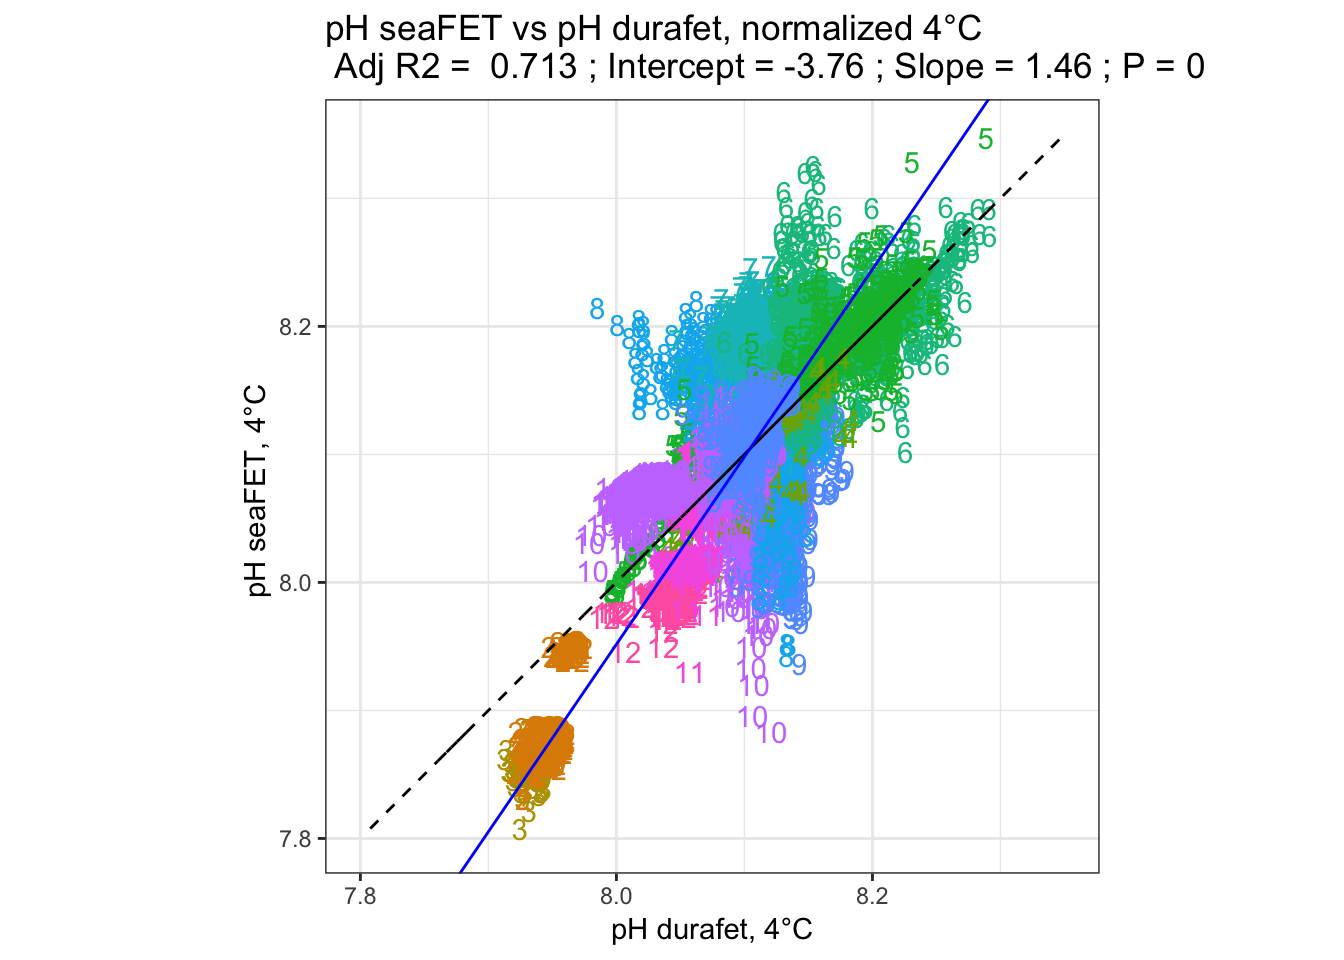
\includegraphics{awipev-CO2_files/figure-latex/pHs comparaison-1.pdf}
\includegraphics{awipev-CO2_files/figure-latex/pHs comparaison-2.pdf}

\hypertarget{calculated-durafet-phs}{%
\subsubsection{\texorpdfstring{\textbf{Calculated / Durafet
pHs}}{Calculated / Durafet pHs}}\label{calculated-durafet-phs}}

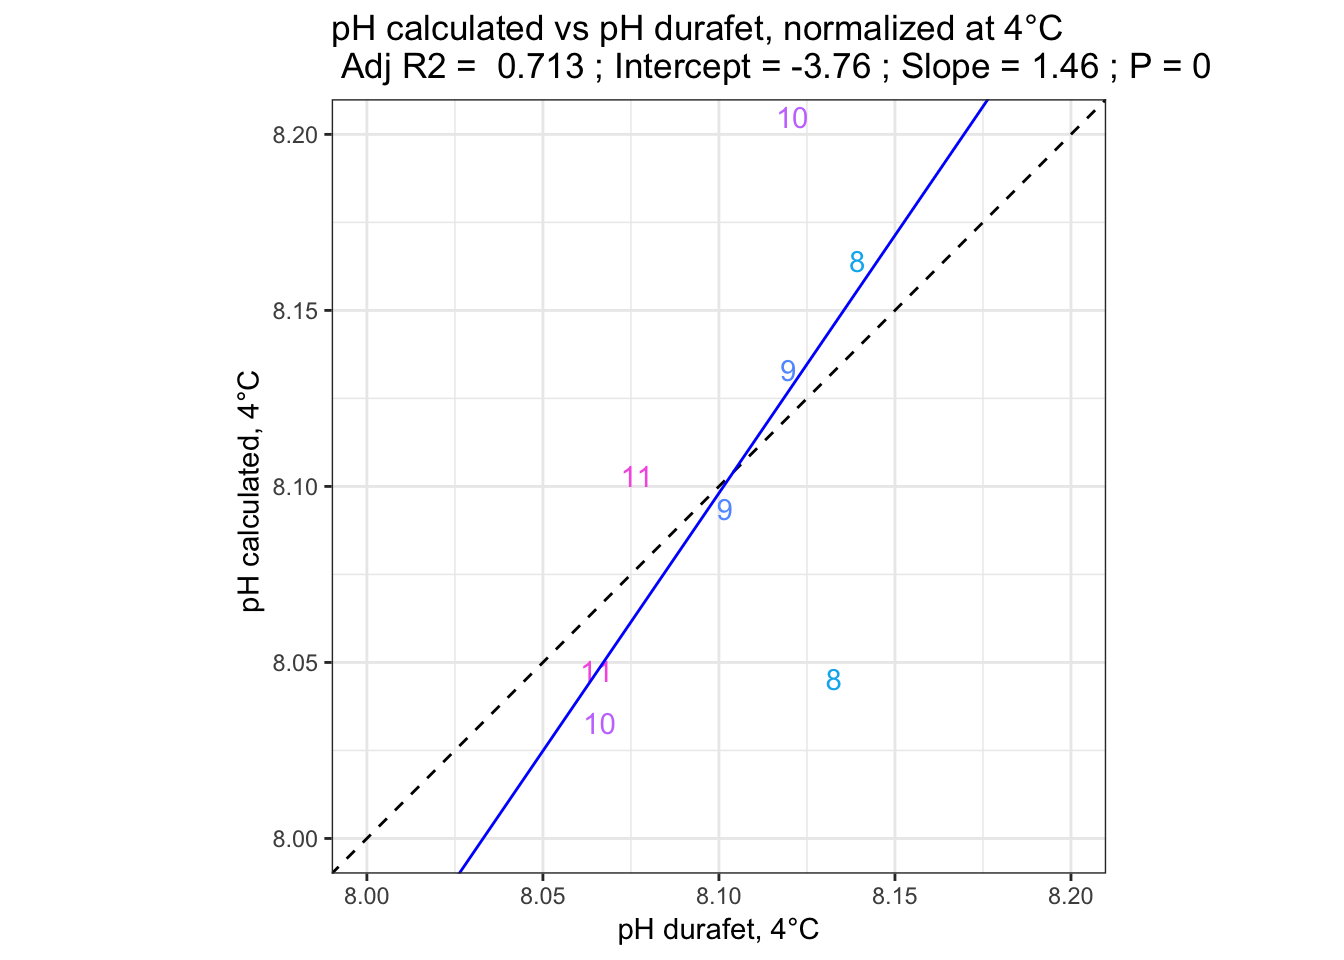
\includegraphics{awipev-CO2_files/figure-latex/pHs comparaison dur calc-1.pdf}

\hypertarget{calculated-seafet-phs}{%
\subsubsection{\texorpdfstring{\textbf{Calculated / seaFET
pHs}}{Calculated / seaFET pHs}}\label{calculated-seafet-phs}}

\includegraphics{awipev-CO2_files/figure-latex/pHs comparaison sf calc-1.pdf}

\hypertarget{spectro-durafet}{%
\subsubsection{\texorpdfstring{\textbf{Spectro /
durafet}}{Spectro / durafet}}\label{spectro-durafet}}

\includegraphics{awipev-CO2_files/figure-latex/pHs comparaison durafet spectro-1.pdf}

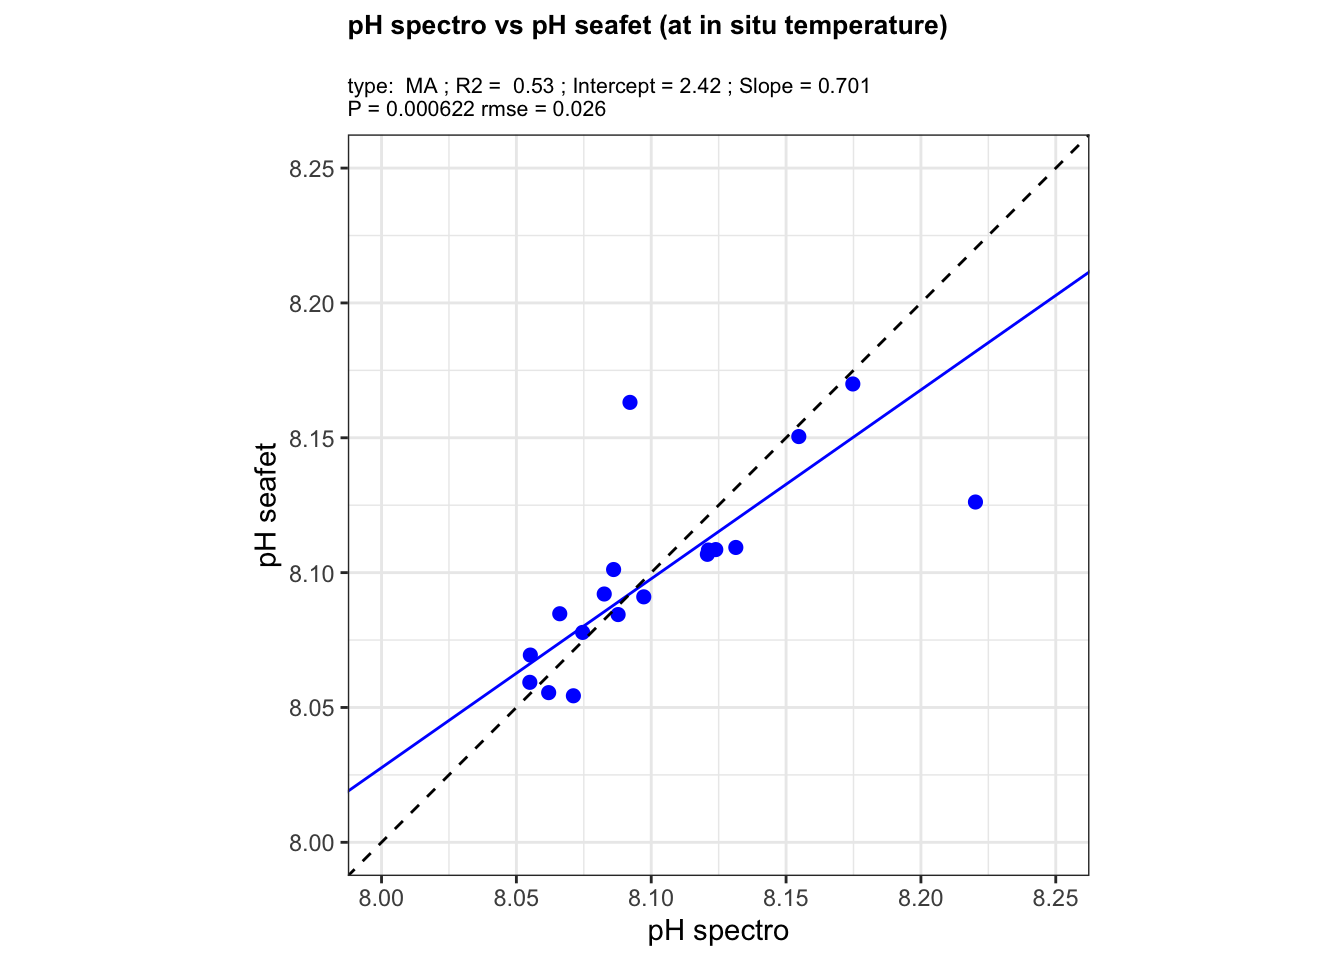
\includegraphics{awipev-CO2_files/figure-latex/pHs comparaison sf spectro-1.pdf}

\hypertarget{snapo-co2}{%
\subsection{SNAPO-CO2}\label{snapo-co2}}

Since November 2018, informations on weekly Ferrybox and monthly
durafet/seaFET samplings are collected in a online document that can be
consulted at anytime:

\href{https://docs.google.com/spreadsheets/d/1bNh9q4bkNoh2ra78XC451EmGb9Q8kMf4ByBnKngeHOg/edit?usp=sharing}{weekly
and monthly samplings}

We found that some analysed discrete seawater replicates for AT/CT,
performed by SNAPO in Paris sometimes show a large difference between
duplicates. Arbitrarily, we decided to take in consideration replicates
with a standard deviation smaller than 10 µmoles.kg-1. In the other case
(greater than 10 µmoles.kg-1), the closest replicate from the general
trend will be kept with qflag\_at/qflag\_ct of 2 (correct analysis) and
the farthest one will be rejected with a flag of 1. There are exceptions
when it is difficult to decide which of the replicates need to be
eliminated.

For TA, dulpicates's flags that have been changed from 2 (good) to 1
(not good) are:

2015-11-18 , 2016-07-28, 2016-09-29, 2016-11-17, 2016-11-23, 2016-12-29,
2017-01-19, 2017-05-04, 2017-08-31, 2018-04-26, 2018-05-04, 2018-05-16,
2018-05-25, 2018-06-22, 2018-06-30, 2018-07-27, 2018-07-20, 2018-08-03,
2018-08-10, 2018-08-24, 2018-08-31, 2018-09-07, 2018-09-14, 2018-09-21,
2018-09-28, 2018-10-05, 2018-10-12, 2018-10-19, 2018-10-26, 2018-11-02,
2018-11-09, 2018-11-16, 2018-11-23, 2019-08-23, 2019-09-20, 2019-11-08,
2019-11-23.

For CT, duplicates's flags that have been changed from 2 (good) to 1
(not good) are:

2015-08-06, 2015-08-13, 2016-05-12, 2016-05-19, 2016-06-16, 2016-07-28,
2016-09-08, 2016-10-27, 2016-11-17, 2017-01-19, 2017-03-02, 2017-04-27,
2017-09-14, 2018-04-26, 2018-05-04, 2018-05-12, 2018-05-25, 2018-06-30,
2018-07-20, 2018-08-03, 2018-08-31, 2018-09-07, 2018-09-14, 2018-09-28,
2018-10-05, 2018-10-12, 2018-10-19, 2018-10-26, 2018-11-02, 2018-11-09,
2018-11-16, 2018-11-23, 2019-05-03, 2019-05-10, 2019-08-23.

Also in the Discrete\_sampling\_AWIPEV.csv, some analysed samples have
been flaged ``3'' by the SNAPO. After a close look, these samples are
not differents from their duplicates. Then we put the flag to ``2''
(good result).

For TA and CT, samples's flags that have been changed from 3 to 2 are:
2019-12-27 (2264 and 2130), 2019-10-25 (2332 and 2152), 2019-09-06 (2268
and 2116).

\includegraphics{awipev-CO2_files/figure-latex/SNAPO-1.pdf}
\includegraphics{awipev-CO2_files/figure-latex/SNAPO-2.pdf}
\includegraphics{awipev-CO2_files/figure-latex/SNAPO-3.pdf}
\includegraphics{awipev-CO2_files/figure-latex/SNAPO-4.pdf}
\includegraphics{awipev-CO2_files/figure-latex/SNAPO-5.pdf}
\includegraphics{awipev-CO2_files/figure-latex/SNAPO-6.pdf}

\hypertarget{impact-of-nutrients}{%
\subsection{Impact of nutrients}\label{impact-of-nutrients}}

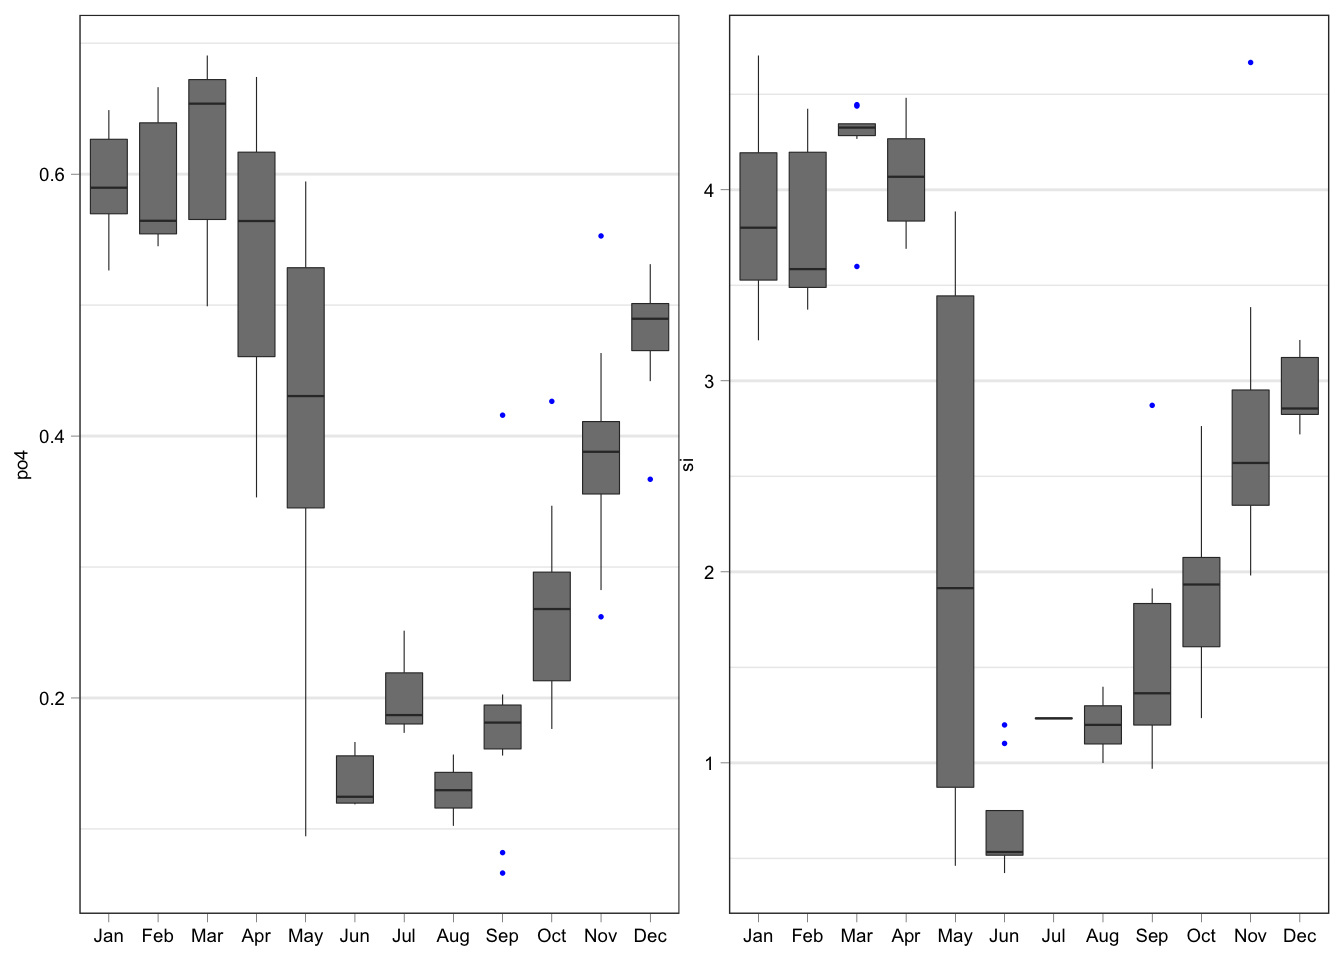
\includegraphics{awipev-CO2_files/figure-latex/impact of nutrients-1.pdf}

The concentration of PO4 and Si varies with a factor 10 along a
composite year. The ranges are respectively, 0.07, 0.69 for PO4 and
0.42, 4.7 for Si.

\hypertarget{using-the-pco2-at-pair-hourly-data}{%
\subsubsection{Using the pCO2-AT pair (hourly
data)}\label{using-the-pco2-at-pair-hourly-data}}

The impact of the min max changes of PO4 on pH, DIC, and Omega\_a are
small: 0.11 mpH units, 0.58 umol/kg for CT and 0 for OmegaAragonite.

The impact of the min max changes of Si on pH, DIC, and Omega\_a are
small: 0.01 mpH units, 0.08 umol/kg for CT and 0 for OmegaAragonite.

\hypertarget{using-the-ct-at-pair-discrete-data}{%
\subsubsection{Using the CT-AT pair (discrete
data)}\label{using-the-ct-at-pair-discrete-data}}

The impact of the min max changes of PO4 on pH, pCO2, and Omega\_a are
small: 1.54 mpH units, -1.18 uatm for pCO2 and 0.01 for OmegaAragonite.

The impact of the min max changes of PO4 on pH, pCO2, and Omega\_a are
small: 0.2 mpH units, -0.16 uatm for pCO2 and 0 for OmegaAragonite.

\hypertarget{impact-of-choice-of-constants}{%
\subsection{Impact of choice of
constants}\label{impact-of-choice-of-constants}}

\begin{longtable}[]{@{}lrrrrrr@{}}
\toprule
flag & S & T & pH & pCO2 & DIC & OmegaAragonite\tabularnewline
\midrule
\endhead
pCO2 and ALK & 34.2 & 3.1 & -0.028 & 0.0 & 3.7 & 0.00\tabularnewline
ALK and DIC & 34.2 & 3.1 & -0.019 & -7.5 & 0.0 & 0.03\tabularnewline
\bottomrule
\end{longtable}

The difference induces by the choice of the carbonic acid constants is
large for pH, pCO2 and DIC and negligible for OmegaAragonite.

\hypertarget{air-sea-co2-flux}{%
\subsection{Air-sea CO2 flux}\label{air-sea-co2-flux}}

To calculate the air-sea CO2 flux, we use:

\begin{itemize}
\tightlist
\item
  seawater pCO2 measured in the FerryBox on water pumped from 11 m
  depth.
\item
  atmospheric CO2 measured at the Zeppelin station and downloaded on
  2020-08-19 from
  \url{https://gaw.kishou.go.jp/search/file/0054-6001-1001-01-01-9999}
\item
  wind spreed data collected by the AWI at 10 m height (sent to JPG by
  P. Fischer, Aug.~2020)
\end{itemize}

Since there are many gaps, a climatological year is used: air-sea flux
calculated by day, then by month, then by year.

seaFET pH is significantly different at the surface and depth. It should
therefore be the same for pCO2.

Let's look first at the stratification (salinity, temperature and
density).

\includegraphics{awipev-CO2_files/figure-latex/stratification-1.pdf}

\begin{longtable}[]{@{}lrrr@{}}
\caption{Median salinity}\tabularnewline
\toprule
montht & median2m & median9m & sal\_range\tabularnewline
\midrule
\endfirsthead
\toprule
montht & median2m & median9m & sal\_range\tabularnewline
\midrule
\endhead
Jan & 34.89 & 34.87 & 0.03\tabularnewline
Feb & 34.96 & 34.94 & 0.01\tabularnewline
Mar & 35.06 & 34.98 & 0.08\tabularnewline
Apr & 35.06 & 35.03 & 0.04\tabularnewline
May & 35.05 & 35.06 & -0.01\tabularnewline
Jun & NA & 35.14 & NA\tabularnewline
Jul & 33.38 & 34.27 & -0.89\tabularnewline
Aug & 33.19 & 34.02 & -0.82\tabularnewline
Sep & 32.39 & 33.10 & -0.70\tabularnewline
Oct & 32.77 & 33.04 & -0.26\tabularnewline
Nov & 33.82 & 33.84 & -0.02\tabularnewline
Dec & 34.21 & 33.58 & 0.63\tabularnewline
\bottomrule
\end{longtable}

\begin{verbatim}
##                         Df Sum Sq Mean Sq F value Pr(>F)    
## tmp$depth                1    122   122.2  142.74 <2e-16 ***
## tmp$montht              11  10634   966.7 1129.10 <2e-16 ***
## tmp$depth:tmp$montht    10    360    36.0   42.06 <2e-16 ***
## Residuals            15235  13044     0.9                   
## ---
## Signif. codes:  0 '***' 0.001 '**' 0.01 '*' 0.05 '.' 0.1 ' ' 1
## 2292 observations deleted due to missingness
\end{verbatim}

\includegraphics{awipev-CO2_files/figure-latex/stratification-2.pdf}
\includegraphics{awipev-CO2_files/figure-latex/stratification-3.pdf}

\begin{longtable}[]{@{}lrrr@{}}
\caption{Median temperature}\tabularnewline
\toprule
montht & median2m & median9m & temp\_range\tabularnewline
\midrule
\endfirsthead
\toprule
montht & median2m & median9m & temp\_range\tabularnewline
\midrule
\endhead
Jan & 0.80 & 0.97 & -0.17\tabularnewline
Feb & -0.68 & -0.53 & -0.15\tabularnewline
Mar & -0.80 & 0.54 & -1.34\tabularnewline
Apr & -0.82 & 1.20 & -2.03\tabularnewline
May & 2.42 & 2.57 & -0.15\tabularnewline
Jun & 3.50 & 3.80 & -0.30\tabularnewline
Jul & 5.60 & 6.05 & -0.44\tabularnewline
Aug & 5.64 & 6.02 & -0.38\tabularnewline
Sep & 4.40 & 4.83 & -0.43\tabularnewline
Oct & 3.10 & 3.60 & -0.50\tabularnewline
Nov & 2.25 & 2.11 & 0.14\tabularnewline
Dec & 1.78 & 1.36 & 0.42\tabularnewline
\bottomrule
\end{longtable}

\begin{verbatim}
##                         Df Sum Sq Mean Sq F value Pr(>F)    
## tmp$depth                1    103     103   68.41 <2e-16 ***
## tmp$montht              11  59928    5448 3621.74 <2e-16 ***
## tmp$depth:tmp$montht    11    929      84   56.16 <2e-16 ***
## Residuals            17526  26363       2                   
## ---
## Signif. codes:  0 '***' 0.001 '**' 0.01 '*' 0.05 '.' 0.1 ' ' 1
\end{verbatim}

\includegraphics{awipev-CO2_files/figure-latex/stratification-4.pdf}

\begin{longtable}[]{@{}lrrr@{}}
\caption{Median density}\tabularnewline
\toprule
montht & median2m & median9m & den\_range\tabularnewline
\midrule
\endfirsthead
\toprule
montht & median2m & median9m & den\_range\tabularnewline
\midrule
\endhead
Jan & 1027.90 & 1027.86 & 0.04\tabularnewline
Feb & 1028.08 & 1028.07 & 0.02\tabularnewline
Mar & 1028.19 & 1028.10 & 0.08\tabularnewline
Apr & 1028.03 & 1028.01 & 0.02\tabularnewline
May & 1027.95 & 1027.96 & -0.01\tabularnewline
Jun & NA & 1027.90 & NA\tabularnewline
Jul & 1026.10 & 1026.99 & -0.89\tabularnewline
Aug & 1026.22 & 1026.73 & -0.51\tabularnewline
Sep & 1025.70 & 1026.19 & -0.49\tabularnewline
Oct & 1026.19 & 1026.29 & -0.10\tabularnewline
Nov & 1026.94 & 1026.97 & -0.03\tabularnewline
Dec & 1027.35 & 1026.97 & 0.38\tabularnewline
\bottomrule
\end{longtable}

\begin{verbatim}
##                         Df Sum Sq Mean Sq F value Pr(>F)    
## tmp$depth                1     69    69.0   133.1 <2e-16 ***
## tmp$montht              11   9017   819.7  1582.1 <2e-16 ***
## tmp$depth:tmp$montht    10    209    20.9    40.4 <2e-16 ***
## Residuals            15235   7893     0.5                   
## ---
## Signif. codes:  0 '***' 0.001 '**' 0.01 '*' 0.05 '.' 0.1 ' ' 1
## 2292 observations deleted due to missingness
\end{verbatim}

\includegraphics{awipev-CO2_files/figure-latex/stratification-5.pdf}
Using the medians because data are missing.

\begin{itemize}
\tightlist
\item
  Salinity
\item
  Temperature is always colder at 0-4 m than below 8 m (0.15 to 2°C).
\end{itemize}

\includegraphics[width=0.03in]{figures/air-sea_CO2_flux}

The annual air-sea CO2 flux is -109 mol/(m2 year).

\hypertarget{maintenance}{%
\subsection{Maintenance}\label{maintenance}}

\hypertarget{remos}{%
\subsubsection{\texorpdfstring{\textbf{REMOS}}{REMOS}}\label{remos}}

\begin{itemize}
\tightlist
\item
  \textbf{2020-09-23}: REMOS started at 20:00 UTC.
\item
  \textbf{2020-09-22}: REMOS stopped at 19:00 UTC because of a power
  shutdown.
\item
  \textbf{2019-03-12}: REMOS on.
\item
  \textbf{2020-02-24}: REMOS off.
\item
  \textbf{2019-09-07}: REMOS back in the water.
\item
  \textbf{2019-09-02}: REMOS removed from the water for maintenance with
  Philipp and Samir.
\item
  \textbf{2018-11-24}: REMOS stopped because of an iceberg. At the
  moment we dont know if instruments are still there/broken.
\end{itemize}

\hypertarget{ferrybox}{%
\subsubsection{\texorpdfstring{\textbf{FerryBox}}{FerryBox}}\label{ferrybox}}

\begin{itemize}
\tightlist
\item
  \textbf{2020-09-30}: FB started at 19:00 UTC.
\item
  \textbf{2020-09-29}: FB stopped at in the morning for few hours.
\item
  \textbf{2020-09-26}: FB stopped at in the morning for few hours.
\item
  \textbf{2020-09-25}: FB stopped at in the morning for few hours.
\item
  \textbf{2020-09-23}: FB started at 20:00 UTC.
\item
  \textbf{2020-09-22}: FB stopped at 19:00 UTC because of a power
  shutdown.
\item
  \textbf{2020-09-22}: FB started again at 08:00 UTC after several
  months of locked down. Lisa repaired it in few minutes only.
\item
  \textbf{2020-09-22}: FB started again after several months of locked
  down. Lisa repaired it in few minutes only.
\item
  \textbf{2020-07-25}: FB stopped. Not possible to go inside to repair
  because the FB is locked after the ``mercurygate''. IPEV locked the FB
  with suspicion of mercury contamination rose up by Bettina
  (Stationleader)
\item
  \textbf{2020-05-24}: FB started again after several months of on
  activity due to very cold T and frozen pipes.
\item
  \textbf{2020-02-18}: FB stopped because of frozen pipes.
\item
  \textbf{2020-01-24}: heater issues in the contenair (power shutdown
  maybe) caused some samples to freeze. See part ``SNAPO'' for details
  on samples.
\item
  \textbf{2019-09-01}: Some interruptions for the FB during 2 weeks of
  maintenance.
\item
  \textbf{2019-06-12}: Markus came to do maintenace.
\item
  \textbf{2019-06-05}: Problem in the relay 15 that controls the waste
  water pump was found. The spare part will be brought here next week
  (when Samir will leave\ldots).
\item
  \textbf{2019-06-03}: Samir is on site alone. Different tests were
  made. Maybe the 2 tapes that feed TA and pCO2 are responsible of the
  problem (low flow).
\item
  \textbf{2019-05-22}: FB is stopped because of several problems.
  Philipp and Marine are working on it.
\item
  \textbf{2019-05-21}: FB is unstable.
\item
  \textbf{2019-04-14}: FB is working again.
\item
  \textbf{2019-04-13}: FB is stopped since 05:00am (the level switch
  stuck in the full position in the waste tank).
\item
  \textbf{2019-02-27}: FB is working again.
\item
  \textbf{2019-02-26}: FB is stopped because of a ``leakage'' issue.
\item
  \textbf{2019-01-17}: FB is stopped until 19th January
\item
  \textbf{2019-01-11}: FB is stopped until 12th Decmeber.
\item
  \textbf{2018-12-28}: FB is stopped until 31st Decmeber.
\item
  \textbf{2018-10-12}: FB is working again.
\item
  \textbf{2018-10-10}: FB is stopped after a seawater leakage.
\item
  \textbf{2018-10-08}: FB is working again.
\item
  \textbf{2018-10-05}: FB is stopped after a seawater leakage.
\item
  \textbf{2018-09-12}: FB is stopped. Problems inland could be the
  reason. The same day Marine make it working again.
\item
  \textbf{2018-04-14}: FB is working again. They made an outlet
  ``by-pass'' tube to flush the seawater directly on the beach, not at
  11 m.
\item
  \textbf{2018-03-08}: Last data at 23:59. Frozen Ferrybox system
  (outlet tubings) in Svalbard, maybe due to a power failure over night
  in Kingsbay. UWO parameters (seaFET and SBE38 are still runing)
\item
  \textbf{2017-05-24}: FerryBox was shut down due to many connexion
  issues\ldots see Philipp's email 24/05/2017 18:17.
\item
  \textbf{2017-03-20}: Philipp arrived in NYA to solve the problem.
\item
  \textbf{2017-03-11}: Iceberg destroyed the power-pumps cables
  (Philipp's email on 2017-03-11 10:40). No more data for all
  parameters.
\item
  \textbf{2017-01-31}: Beginning of the 14-days FB maintenance by
  Philipp and Uwe. Gaps in data could be present during this period.
\item
  \textbf{2017-01-17}: Ferrybox stopped for unknown reasons from
  2017-01-17 21:00 to 2017-01-19.
\item
  \textbf{2016-09-24}: No data because of maintenance until the 28th.
  Except for TA wich has data available for this period.
\item
  \textbf{2016-09-20}: Test in the Ferrybox with the seawater. Seawater
  was ``sucked'' (not pumped) from 7:40 to 10:00 by a vaccum system in
  order to test it. This system was installed if the pumps 1 and 2 broke
  during winter. This is a ``plan C''. This system is not automatic and
  we will be informed about its power up in case of emergency. As long
  as the water is not pumped with this system, we have to monitor the
  data because changements in gas partial pressure can occur.
\item
  \textbf{2016-09-12}: No data because of maintenance until the 18th.
\item
  \textbf{2016-09-10}: No data because of maintenance until the 11th.
\item
  \textbf{2016-05-09}: data are back.
\item
  \textbf{2016-05-04}: No data for all parameters because of electricity
  issues.
\item
  \textbf{2016-04-23}: FerryBox was shut down by AWI team for
  maintenance.
\item
  \textbf{2016-02-23}: FerryBox was switched on by AWI team after
  maintenance.
\item
  \textbf{2015-12-20}: FerryBox was shut down because of pump issues.
  Waiting for the maintenance in February.
\item
  \textbf{2015-11-27}: The ferrybox was down from Nov.~18th until today
  Nov.~27th. (emails from P.Fischer 2015-11-24 23:09 and Station Leader
  AWIPEV 2015-11-27 12:57). Tubes frozen.
\end{itemize}

\hypertarget{ta-analyser}{%
\subsubsection{\texorpdfstring{\textbf{TA
analyser}}{TA analyser}}\label{ta-analyser}}

\begin{itemize}
\tightlist
\item
  \textbf{2019-11-15}: TA calibration done by Gwendall is OK but the
  sensore seems to have problem since 2019-10-16. Video conference is
  scheduled with Steffen on 2019-11-19. Maybe sample supply is
  defective.
\item
  \textbf{2019-07-12}: Steffen told us that calibration was not OK. To
  check it, he calculated the mediane of the pH/volume sample /
  volumeIndicatorfactor and compared them to January/October
  calibration. We wait for Steffen recommandations before to make
  another calibration.
\item
  \textbf{2019-06-07}: Samir did the TA calibration: T0 with CRM 145.
  Beginning of a 3-months period. TA was stable before the calibration
  and calibration was OK.
\item
  \textbf{2019-02-15}: No data from 15th (14:08:21 UTC) to 19th February
  (14:58:46 UTC). files transfered but no data. No explanation.
\item
  \textbf{2019-01-26}: Philipp did the TA calibration: T0 with CRM 145.
  Beginning of a 3-months period. Flow filter was also lifted up and the
  seawater flow has therefore increased.
\item
  \textbf{2019-01-16}: Bad data since this date.
\item
  \textbf{2018-12-28}: HCL and BCG cartridges were changed by Marine.
\item
  \textbf{2018-11-26}: TA analyser was stopped in order to save reagents
  because of filter issues.
\item
  \textbf{2018-11-20}: A web interface was created by KM Contros to
  access the TA via VPN and Virtual Machine (VNC viewer). Samir received
  password and access from the AWI in order to communicate from France
  with the TA.
\item
  \textbf{2018-10-31}: New TA analyser (SN 0317-001) was installed with
  a new membrane inside (completely new technology). Tests were made
  with Steffen from KM Contros.
\item
  \textbf{2018-07-31}: TA analyser was received (SN TA-1215-001) and
  pluged again. First data were received (high: 2450 and low: 2150) but
  salinity issue since this time. Uwe/Philipp try to find if this comes
  from comunication issue with the FB.
\item
  \textbf{2018-06-20}: TA analyser was stopped in order to save reagents
  because leakage in degasing unit is not solved. Email was sent to
  Steffen.
\item
  \textbf{2018-01-05}: TA analyser switched on and first communication
  tests. S/N TA-0317-001.
\item
  \textbf{2017-08-23}: The 2 TA analysers were sent to Contros for
  repair, 1 will be sent back to NYA after. No more TA data during this
  period.
\item
  \textbf{2017-04-06}: (12:30 UTC) Christelle repaired TA analyser by
  removing air bubbles in Acid tubings (advices from Steffen).
\item
  \textbf{2017-04-01}: No more TA data\ldots waiting for a diagnostic by
  Contros.
\item
  \textbf{2017-03-31}: (11:00 UTC) Christelle switched on TA analyser.
\item
  \textbf{2017-03-30}: (07:30 UTC) Christelle switched TA analyser on
  ``standby'' because of cartridge leakage issue (3 ways connector
  broken).
\item
  \textbf{2017-03-21}: Philipp changed the TA analyser provided by
  Contros.
\item
  \textbf{2017-02-10}: TA cleaning salt crusts.
\item
  \textbf{2017-02-09}: TA calibration with CRM at 12:20.
\item
  \textbf{2017-01-20}: The date issue with TA analyser since 201-01-07
  was fixed by Uwe with a restart of the Ferrybox Module around 14:00
  UTC.
\item
  \textbf{2016-11-15}: TA calibration done by Christelle with Dickson
  CRM run as regular sample (measure mode). Data of this calibration do
  not appear on plot because TA analyser is disconnected from the
  FerryBox.
\item
  \textbf{2016-09-16}: Cleaning of the TA analyser removing all the salt
  crusts from the bottom of the degazing unit (Samir).
\item
  \textbf{2016-06-24}: BCG cartridge was changed (Christelle, ObsEng).
\item
  \textbf{2016-05-31}: HCL cartridge was changed (Christelle, ObsEng).
\item
  \textbf{2016-05-01}: No data for TA.
\item
  \textbf{2016-04-26}: Salt crusts inside the TA analyser appeared
  during deployment (see pictures) were removed by René Burgi
  (Observatory engineer) according to Contros advices (email from
  Steffen Assmann 13/04/2016 10:30).
\end{itemize}

\hypertarget{ph-seafet-1}{%
\subsubsection{\texorpdfstring{\textbf{pH
seaFET}}{pH seaFET}}\label{ph-seafet-1}}

\begin{itemize}
\tightlist
\item
  \textbf{2019-09-02}: Out from the water for maintenance and cleaning
  only.
\item
  \textbf{2018-04-17}: seaFET \#1005 was changed on the REMOS and seaFET
  \#007 (from Villefranche) was installed. Continuous mode with external
  power supply was set and internal pack of baterries was removed. Old
  seaFET will be brought back to France with Samir.
\item
  \textbf{2018-03-09}: \#007 seaFET currently in USA will be sent by
  seabird to NYA. \#1005 seaFET currently in NYA will be sent to USA for
  update, following all external issues, for free.
\item
  \textbf{2017-08-24}: seaFET \#1005 was installed on the REMOS into the
  field.
\end{itemize}

\hypertarget{cross-flow-filter}{%
\subsubsection{\texorpdfstring{\textbf{Cross-Flow
filter}}{Cross-Flow filter}}\label{cross-flow-filter}}

\begin{itemize}
\tightlist
\item
  \textbf{2019-01-26}: The filter was lifted up in order to fix the flow
  problem.
\item
  \textbf{2018-11-01}: The filter clogged a lot of time even after acid
  cycles. It was not replaced since its initial installation with the TA
  analyser. We think to replace it soon.
\item
  \textbf{2016-07-20}: Cross filter was cleanned by Obs. eng. with 10-15
  min tape water flush.
\end{itemize}

\hypertarget{durafet}{%
\subsubsection{\texorpdfstring{\textbf{durafet}}{durafet}}\label{durafet}}

\begin{itemize}
\tightlist
\item
  \textbf{2019-09-05}: same durafet
\item
  \textbf{2017-10-30}: (13:00 UTC) Durafet holder was changed by Benoit
  and the new one (made by Uwe) more larger (all the durafet's body is
  plunge in the seawater) was installed.
\item
  \textbf{2017-08-24}: durafet was installed.
\end{itemize}

\hypertarget{pco2-1}{%
\subsubsection{\texorpdfstring{\textbf{\emph{p}CO\textsubscript{2}}}{pCO2}}\label{pco2-1}}

\begin{itemize}
\tightlist
\item
  \textbf{2019-09-03}: \emph{p}CO\textsubscript{2} analyser (S/N:
  CO2FT-0515-001) have been installed and \emph{p}CO\textsubscript{2}
  analyser (S/N: CO2FT-0215-001) was sent to Kiel for calibration.
\item
  \textbf{2018-10-31}: \emph{p}CO\textsubscript{2} analyser (S/N:
  CO2FT-0215-001) have been installed and \emph{p}CO\textsubscript{2}
  analyser (S/N: CO2FT-0515-001) was brought back to France and waiting
  2019 fundings to bring it for calibration.
\item
  \textbf{2018-04-16}: \emph{p}CO\textsubscript{2} analyser switching by
  Uwe and Samir. S/N CO2FT-0515-001 is now installed. Old
  \emph{p}CO\textsubscript{2} sensor will be brought back to France with
  Samir.
\item
  \textbf{2017-02-07}: pCO2 analyser switching by Uwe. S/N
  CO2FT-0215-001 is now installed.
\item
  \textbf{2016-09-13}: Changement of the \emph{p}CO\textsubscript{2} S/N
  CO2FT-0515-001 membrane (Uwe from 4H-Jena).
\item
  \textbf{2016-02-28}: \emph{p}CO\textsubscript{2} analyser (S/N
  CO2FT-0215-001) was sent to calibration and the second
  \emph{p}CO\textsubscript{2} analyser (S/N: CO2FT-0515-001) have been
  installed.
\end{itemize}

\hypertarget{script-data}{%
\subsection{Script + data}\label{script-data}}

Here is reported all important modifications made on
\emph{ny-alesund\_cc.}. All documents concerning maintenance, tasks to
do, calibration\ldots{} are accessible by the AWIPEV staff on this link
with special access:

\href{https://spaces.awi.de}{wiki document}

\href{https://docs.google.com/spreadsheets/d/1bNh9q4bkNoh2ra78XC451EmGb9Q8kMf4ByBnKngeHOg/edit\#gid=1034421443}{Logbook
discrete sampling}

\href{https://docs.google.com/spreadsheets/d/1QwAJm7TttoEwue-CUM0efhqEAMwj5m148Gy_Mp-1maM/edit?ts=5ed0fca6\#gid=2036495380}{Logbook
FerryBox}

\href{https://docs.google.com/spreadsheets/d/1arKYfUjmg3YrgQ5g9LN_XFwUORyz7nqlKNWq3uYok3U/edit?ts=5c7e1d16\#gid=393659093}{UWO-Ferrybox
variables from our sensors}

\href{https://dashboard.awi.de/?dashboard=3760}{Dashboard}

\href{https://spaces.awi.de/confluence/display/MOS/NRT+data+download+procedures}{Procedure
to download NRT data}

\href{https://dashboard.awi.de/data-xxl/}{AWI NRT database}, search for
svluwobs

\href{https://dashboard.awi.de/?dashboard=9736}{Quick overview AWI NRT
database}

\hypertarget{ferrybox-1}{%
\subsubsection{\texorpdfstring{\textbf{FerryBox}}{FerryBox}}\label{ferrybox-1}}

\begin{itemize}
\tightlist
\item
  \textbf{2020-03-13}: Salinity was filtered above 28 in d\_all.rds
  file.
\item
  \textbf{2018-11-14}: One instrument was removed by Uwe (Chlorophyl-a),
  that means that one column (CHl\_A\_Cyclops) was also removed from the
  Ferrybox data file. Script was modified in consequence.
\end{itemize}

\hypertarget{ph-seafet-2}{%
\subsubsection{\texorpdfstring{\textbf{pH
seaFET}}{pH seaFET}}\label{ph-seafet-2}}

\begin{itemize}
\tightlist
\item
  \textbf{2018-08-30}: voltINT + phINT were filtered from 2017-12-14 to
  2018-01-08 and bad data were removed from 2018-01-08 to 2018-02-02. pH
  spectro from 2018-04-16 07:00:00 was fitted with a mean of 4 days of
  voltINT in order to make the calibration for this 5th period.
\item
  \textbf{2018-07-30}: Flag location (location\_flag) is added in the
  script to localize seaFET/durafet discrete samples: flag 1 = at the
  harbor (not taken in consideration) and flag 0 = in the FB for durafet
  or on site for seaFET (takken in consideration as ``normal''
  sampling"). See seaFET part.
\item
  \textbf{2018-02-02}: Based on Darrell's advices (SeaBird), Philipp
  implemented the seaFET as: 1h periodic sampling with the following
  commands: perdival 1h, navg 5, brstsize 1, opermode periodic.
\item
  \textbf{2017-12-29}: ``SVL\_20171218\_010426.dat'' from seaFet data
  was deleted because of bug with its size (0 octect). pH filter was
  added to ``ny\_alesund\_cc'' file for seaFet data (\textless7.5 and
  \textless8.5).
\end{itemize}

\hypertarget{durafet-1}{%
\subsubsection{\texorpdfstring{\textbf{Durafet}}{Durafet}}\label{durafet-1}}

\begin{itemize}
\tightlist
\item
  Reference spectro measurement from the 2019-01-18 11:00 do not match
  with a durafet raw data because Ferrybox was off. This reference point
  was not takken in consideration for calibration. The window of the
  previous and next calibration periods was extended.
\end{itemize}

\hypertarget{pco2-2}{%
\subsubsection{\texorpdfstring{\textbf{\emph{p}CO\textsubscript{2}}}{pCO2}}\label{pco2-2}}

\begin{itemize}
\tightlist
\item
  \textbf{2020-03-11}: Post calibration parameters for period 4
  (2018-04-16 to 2018-10-31) were not taken in consideration because
  they lead to wrong correction.
\item
  \textbf{2019-11-18}: Calibration parameters from \#0215-001 were added
  to ``server\ldots/data/NRT\_data/Data\_Processing\_sheet\_pCO2.csv''
  (new path).
\item
  \textbf{2018-08-29}: Calibration parameters from \#0215-001 were added
  to ``./data/Calibration\_pCO2/Data\_Processing\_sheet\_pCO2.csv''.
\item
  \textbf{2018-04-20}: For \emph{p}CO\textsubscript{2} Calibration the
  previous period (N° 4) was added to the script ``ny-alesund\_cc'' line
  466.
\item
  \textbf{2015-10-13}: we put back the spike.pCO2 to 600 because data in
  October reached more than 350 µAtm. We let this like that and we are
  going to deal with it manually later if needed.
\item
  \textbf{2015-09-28}: we put the spike.pCO2 (detection of peaks:
  threshold) at 350 to remove anomalies on the 12 and 15 September. We
  have to monitor data. If data reach this value, then problem.
\end{itemize}

\hypertarget{snapo}{%
\subsubsection{\texorpdfstring{\textbf{SNAPO}}{SNAPO}}\label{snapo}}

\begin{itemize}
\item
  \textbf{2020-01-23}: Freezed and lost samples because of heater issue
  in the container: 15/11/2019 (durafet x1), 03/12/2019 (FB x2),
  11/12/2019 (FB x2), 13/12/2019 (FB x2), 20/12/2019 (FB x2), 03/01/2020
  (FB x2). Following samples could have been frozen, not sure:
  06/09/2019 (FB x2), 13/09/2019 (seaFET x1), 13/09/2019 (FB x2),
  20/09/2019 (FB x1), 27/09/2019(FB x2), 04/10/2019 (FB x2), 11/10/2019
  (FB x1), 11/10/2019 (durafet x1), 25/10/2019 (FB x2), 01/11/2019 (FB
  x1), 15/11/2019 (FB x1).
\item
  \textbf{2020-01-15}: Results from 2019-04-19 to 2019-08-31 (sent in
  September 2019) were received. FB duplicates from 2019-08-09 were
  analysed as Durafet because of wrong box. One sample from 2019-06-07
  (durafet) was analysed by Paris because of wrong box.
\item
  \textbf{2019-04-30}: Duplicate ``Ferrybox'' samples (SN0316 and SN264,
  2019-02-22 14:05) were sent by mistake in Villefranche for pH
  measurements. Those results were put in the datafile as ``durafet''
  samples as soon as they are comming from the Ferrybox tape seawater.
  We will add a lack of DIC for this week. TA will be measured in
  Villefranche.
\item
  \textbf{2018-08-30}: flag of 1 AT duplicate (2205) from 2017-08-31 was
  put to 3 (dosage douteux).
\end{itemize}

\hypertarget{files---server}{%
\subsubsection{\texorpdfstring{\textbf{Files -
server}}{Files - server}}\label{files---server}}

\begin{itemize}
\tightlist
\item
  \textbf{2019-11-15}: Script including the new data downloading from
  the NRT AWI database is running (ny-alesund\_cc.R). From this date,
  data are donwloaded from AWI NRT dtabase. We are waiting some setting
  from Philipp to have the entire dataset. Only 2018-2019 are available
  for the moment. New path was created in the server and pCloud/exp168
  with ``NRT\_data'' file. Please see the picture bellow.
\item
  \textbf{2018-04-19}: Since ``Ferrybox'' is on again, the adding to
  solve the files issues are making not data into d\_hour for this
  period (2018-09-03 to 2018-14-04). This adding was put in comments
  now. In seaFET data reading, S/N have been changed from 1005 to 0007.
\item
  \textbf{2018-03-21}: Files issues. FerryBox instruments are down
  because of freezing but UWO instrument as seaFET and SBE38 are OK.
  Removing of one 0 octet file from seaFET20180317\_1404 and put back
  seaFET files from 20180309 to 20180312 in seaFET folder. They were in
  SBE38 folder\ldots Weird. Additionnal script lines were added in order
  to deal with the issue of ``in situ'' created date whereas
  ``Ferrybox'' created data ware not. Since ``in situ'' parameters are
  running (d df) and not ``in ferrybox'' parameters (z df), the new
  datetime lines are not taking in consideration with the left\_join
  function we have to add them during Ferrybox shutdown.
\item
  \textbf{2018-03-09}: Script issue solved with first negative values
  encountred in SBE38 files. We find a regex solution to take ``space +
  space or negative value'' in consideration.
\item
  \textbf{2017-11-07}: Wrong seaFET files (wrong datetime starting on
  the 5th September) from 24 to 26 October were fixed. File
  ``SVL\_20171024\_030426\_to\_20171026\_110425\_SeaFet-1005.txt'' were
  created in SeaFet\_archive.
\end{itemize}

\hypertarget{data-processing}{%
\subsubsection{Data processing}\label{data-processing}}

\hypertarget{script-ny-alesund_cc.r-which-runs-on-awipevawipev-co2.obs-vlfr.fr}{%
\paragraph{\texorpdfstring{Script ny-alesund\_cc.R which runs on
\href{mailto:awipev@awipev-co2.obs-vlfr.fr}{\nolinkurl{awipev@awipev-co2.obs-vlfr.fr}}}{Script ny-alesund\_cc.R which runs on awipev@awipev-co2.obs-vlfr.fr}}\label{script-ny-alesund_cc.r-which-runs-on-awipevawipev-co2.obs-vlfr.fr}}

\begin{itemize}
\tightlist
\item
  reads data from the AWI NRT database
  \href{https://dashboard.awi.de/?dashboard=9736}{Quick overview AWI NRT
  database}
\item
  calibrates pCO2 data
\item
  data cleaning:

  \begin{itemize}
  \tightlist
  \item
    Argo Global Range Test.
  \item
    filter salinities above 28
  \item
    filter temperatures above 10
  \item
    filter seaFET Volt (outliers)
  \item
    filter seaFET pH (outliers)
  \item
    filter durafet (outliers)
  \end{itemize}
\item
  Quality flags

  \begin{itemize}
  \tightlist
  \item
    1: good data
  \item
    3: impossible date and time test
  \item
    4: data not usable according to manufacturer (flush mode, zero mode,
    calibration mode\ldots)
  \item
    6: failing the manufacturer range test (not used)
  \item
    7: failing the regional range test
  \item
    12: failing the spike test (NAs from despike)
  \item
    13: failing the gradient test
  \item
    15: the instrument was not deployed or operated
  \item
    16: acid flush
  \item
    99: failing the final visual inspection of the data.
  \end{itemize}
\item
  Despike using oce::despike with n=2, k=5761
\item
  Files generated:

  \begin{itemize}
  \tightlist
  \item
    previous\_NRT\_data.rds: all NRT data without alteration from the
    beginning (2015)
  \item
    all\_nydata\_minute.rds: all data after filtering and despike
    describe above (every minute)
  \item
    all\_nydata\_hour.rds: hourly means of all data after filtering and
    despike describe above (every minute)
  \item
    nydata\_minute.rds: selected data after filtering and despike
    describe above (every minute). \textbf{Useful?}
  \item
    nydata\_hour.rds: selected hourly means of all data after filtering
    and despike describe above (every minute). This is for further data
    processing.
  \end{itemize}
\end{itemize}

\hypertarget{script-awipev-co2.rmd-which-runs-locally}{%
\paragraph{Script awipev-co2.Rmd which runs
locally}\label{script-awipev-co2.rmd-which-runs-locally}}

\begin{itemize}
\tightlist
\item
  reads locally
  fb\_awipev-co2\_server/ny-alesund/data/NRT\_data/nydata\_hour.rds
\item
  sal\_mix: when ferrybox data (sal\_fb) are missing, they are replaced
  by data from the profiling ctd for depths \textgreater{} 8 m
  (sal\_insitu\_ctd\_9m)
\item
  temp\_mix: when data of in situ temperature at 11 m
  (temp\_insitu\_11m) are missing, they are replaced by data from the
  profiling ctd for depths \textgreater{} 8 m
\item
  pco2\_calc\_fb: pco2 calc from AT/CT ferrybox = carb avec temp\_fb
  +sal\_fb
\item
  calibrate seafet pH

  \begin{itemize}
  \tightlist
  \item
    ph\_s\_sf\_temp\_insi: pH spectro seaFET pH insi calculé avec AT
    interpolée + temp\_mix +sal\_mix
  \item
    E0int25\_sf: calculé à partir du voltage interne +
    ph\_s\_sf\_temp\_insi (temp 11m + temp\_insitu\_ctd\_9m si trous) +
    temp CTD 9m + sal CTD 9m (calib seaFET fonction 1)
  \item
    phint\_tot\_sf: calculé à partir du voltage interne + E0 + temp CTD
    + sal CTD (calib seaFET fonction 2)
  \end{itemize}
\item
  ph\_calc: pH calc from AT/CT ferrybox = carb avec temp\_fb +sal\_fb
\item
  despike pH seaFET
\item
  calibrate durafet pH

  \begin{itemize}
  \tightlist
  \item
    ph\_s\_dur\_temp\_fb: pH spectro durafet pH insi calculé avec AT
    interpolée + temp\_fb +sal\_fb
  \end{itemize}
\item
  Relation at / sal\_mix
\item
  at\_calc: calculé from sal\_mix
\item
  saves locally d\_all.rds which comprises all variables plus those
  generated in the script
\end{itemize}

\hypertarget{villefranche-server-informations}{%
\subsubsection{Villefranche Server
informations}\label{villefranche-server-informations}}

\begin{itemize}
\tightlist
\item
  Serveur : awipev-co2 (193.50.85.104)
\item
  3 comptes: awipev (partagé avec Samir), gattuso, nydata (pour l'envoi
  des données par P. Fischer mais n'est plus utilisé).
\item
  Pour se connecter à awipev-co2.obs-vlfr.fr

  \begin{itemize}
  \tightlist
  \item
    ssh
    \href{mailto:awipev@awipev-co2.obs-vlfr.fr}{\nolinkurl{awipev@awipev-co2.obs-vlfr.fr}}
  \end{itemize}
\item
  Intervention sur le serveur :

  \begin{itemize}
  \tightlist
  \item
    ssh
    \href{mailto:awipev@awipev-co2.obs-vlfr.fr}{\nolinkurl{awipev@awipev-co2.obs-vlfr.fr}}
  \item
    rebooting Ubuntu server: sudo shutdown -r now
  \item
    to check versions:

    \begin{itemize}
    \tightlist
    \item
      dpkg -l \textbar{} grep shiny
    \item
      dpkg -l \textbar{} grep r-base
    \end{itemize}
  \item
    To update Ubuntu, R and its packages:

    \begin{itemize}
    \tightlist
    \item
      sudo su
    \item
      apt-get upgrade
    \end{itemize}
  \item
    To restart shiny server: sudo systemctl restart shiny-server

    \begin{itemize}
    \tightlist
    \item
      update shiny server: follow procedure detailed on the shiny web
      page Data processing
    \end{itemize}
  \end{itemize}
\item
  To install R packages:

  \begin{itemize}
  \tightlist
  \item
    ssh
    \href{mailto:gattuso@awipev-co2.obs-vlfr.fr}{\nolinkurl{gattuso@awipev-co2.obs-vlfr.fr}}
  \item
    sudo R (then password)
  \item
    install.packages(``tidyverse'')
  \end{itemize}
\end{itemize}

\textbf{crontab
\href{mailto:awipev@awipev-co2.obs-vlfr.fr}{\nolinkurl{awipev@awipev-co2.obs-vlfr.fr}}}

Si on veut remplacer intégralement les fichiers de pCloud par ceux de
awipev-co2 : ajouter ``--delete'' à la commande rsync. Pattern des
commandes : \# m h dom mon dow command

\begin{itemize}
\tightlist
\item
  (Every 4 hour on the hour, a crontab action runs automatically the
  script ny-alesund/R/ny-alesund\_cc.R. This script essentially appends
  the daily files from AWI-NRT database and cleans the data)

  \begin{itemize}
  \tightlist
  \item
    00 \emph{//1 } * * cd \$HOME; USER=awipev R --vanilla \textless{}
    ny-alesund/R/ny-alesund\_cc.R \textgreater{}
    ny-alesund/R/log\_ny-alesund\_cc.txt 2\textgreater\&1
  \end{itemize}
\item
  (Every 4 hour at 10 min past the hour, the web page is generated)

  \begin{itemize}
  \tightlist
  \item
    10 \emph{//1 } * * cd web; USER=awipev bash awipev-co2.sh
    \textgreater{} awipev-web.log 2\textgreater\&1
  \end{itemize}
\item
  (At 05:00 the files from server/web are copied to gattuso's iMac in
  pCloud \ldots{} Exp168)

  \begin{itemize}
  \tightlist
  \item
    00 05 * * * /usr/bin/rsync -e ``ssh -o StrictHostKeyChecking=no''
    -avh /home/awipev/web
    `\href{mailto:gattuso@gattuso.obs-vlfr.fr}{\nolinkurl{gattuso@gattuso.obs-vlfr.fr}}:/Users/gattuso/pCloud~Sync/Documents/experiments/exp168\_awipev-CO2/fb\_awipev-co2\_server/'
  \end{itemize}
\item
  (At 05:00 the files from server/ny-alesund are copied to gattuso's
  iMac in pCloud/Exp168)

  \begin{itemize}
  \tightlist
  \item
    00 05 * * * /usr/bin/rsync -e ``ssh -o StrictHostKeyChecking=no''
    -avh /home/awipev/ny-alesund
    `\href{mailto:gattuso@gattuso.obs-vlfr.fr}{\nolinkurl{gattuso@gattuso.obs-vlfr.fr}}:/Users/gattuso/pCloud~Sync/Documents/experiments/exp168\_awipev-CO2/fb\_awipev-co2\_server/'
  \end{itemize}
\end{itemize}

\hypertarget{web-page}{%
\subsubsection{Web page}\label{web-page}}

\begin{itemize}
\item
  La page web index.html est faite sur le serveur awipev/web grâce au
  script awipev-CO2\_web.Rmd puis transférée et renommée dans
  awipev/awipev-CO2\_web
\item
  Création du répertoire web qui contient ce qu'il faut pour générer la
  page web:

  \begin{itemize}
  \tightlist
  \item
    AWIPEV-Logo.jpg
  \item
    Discrete\_sampling\_AWIPEV.csurv
  \item
    awipev-CO2\_web.Rmd
  \item
    awipev-co2.sh (lancer par bash awipev-co2.sh)
  \end{itemize}
\item
  Accessible \url{https://awipev-co2.obs-vlfr.fr}
\item
  On utilise un shell script awipev-co2.sh :

  \#!/bin/bash

  \# script de lancement via crontab echo `---------deb awipev-co2.sh
  -----------'

  \# On lance la fabrication du html (une seule ligne) cd web; R -e
  `library(``rmarkdown'');library(``knitr'');rmarkdown::render(``awipev-CO2\_web.Rmd'')';
  cp awipev-CO2\_web.html ../awipev-CO2\_web/index.html

  echo `---------fin awipev-co2.sh -----------'
\end{itemize}

A la main dans le terminal, cela donne :

\begin{itemize}
\tightlist
\item
  ssh
  \href{mailto:awipev@awipev-co2.obs-vlfr.fr}{\nolinkurl{awipev@awipev-co2.obs-vlfr.fr}}
\item
  cd; bash web/awipev-co2.sh
\end{itemize}

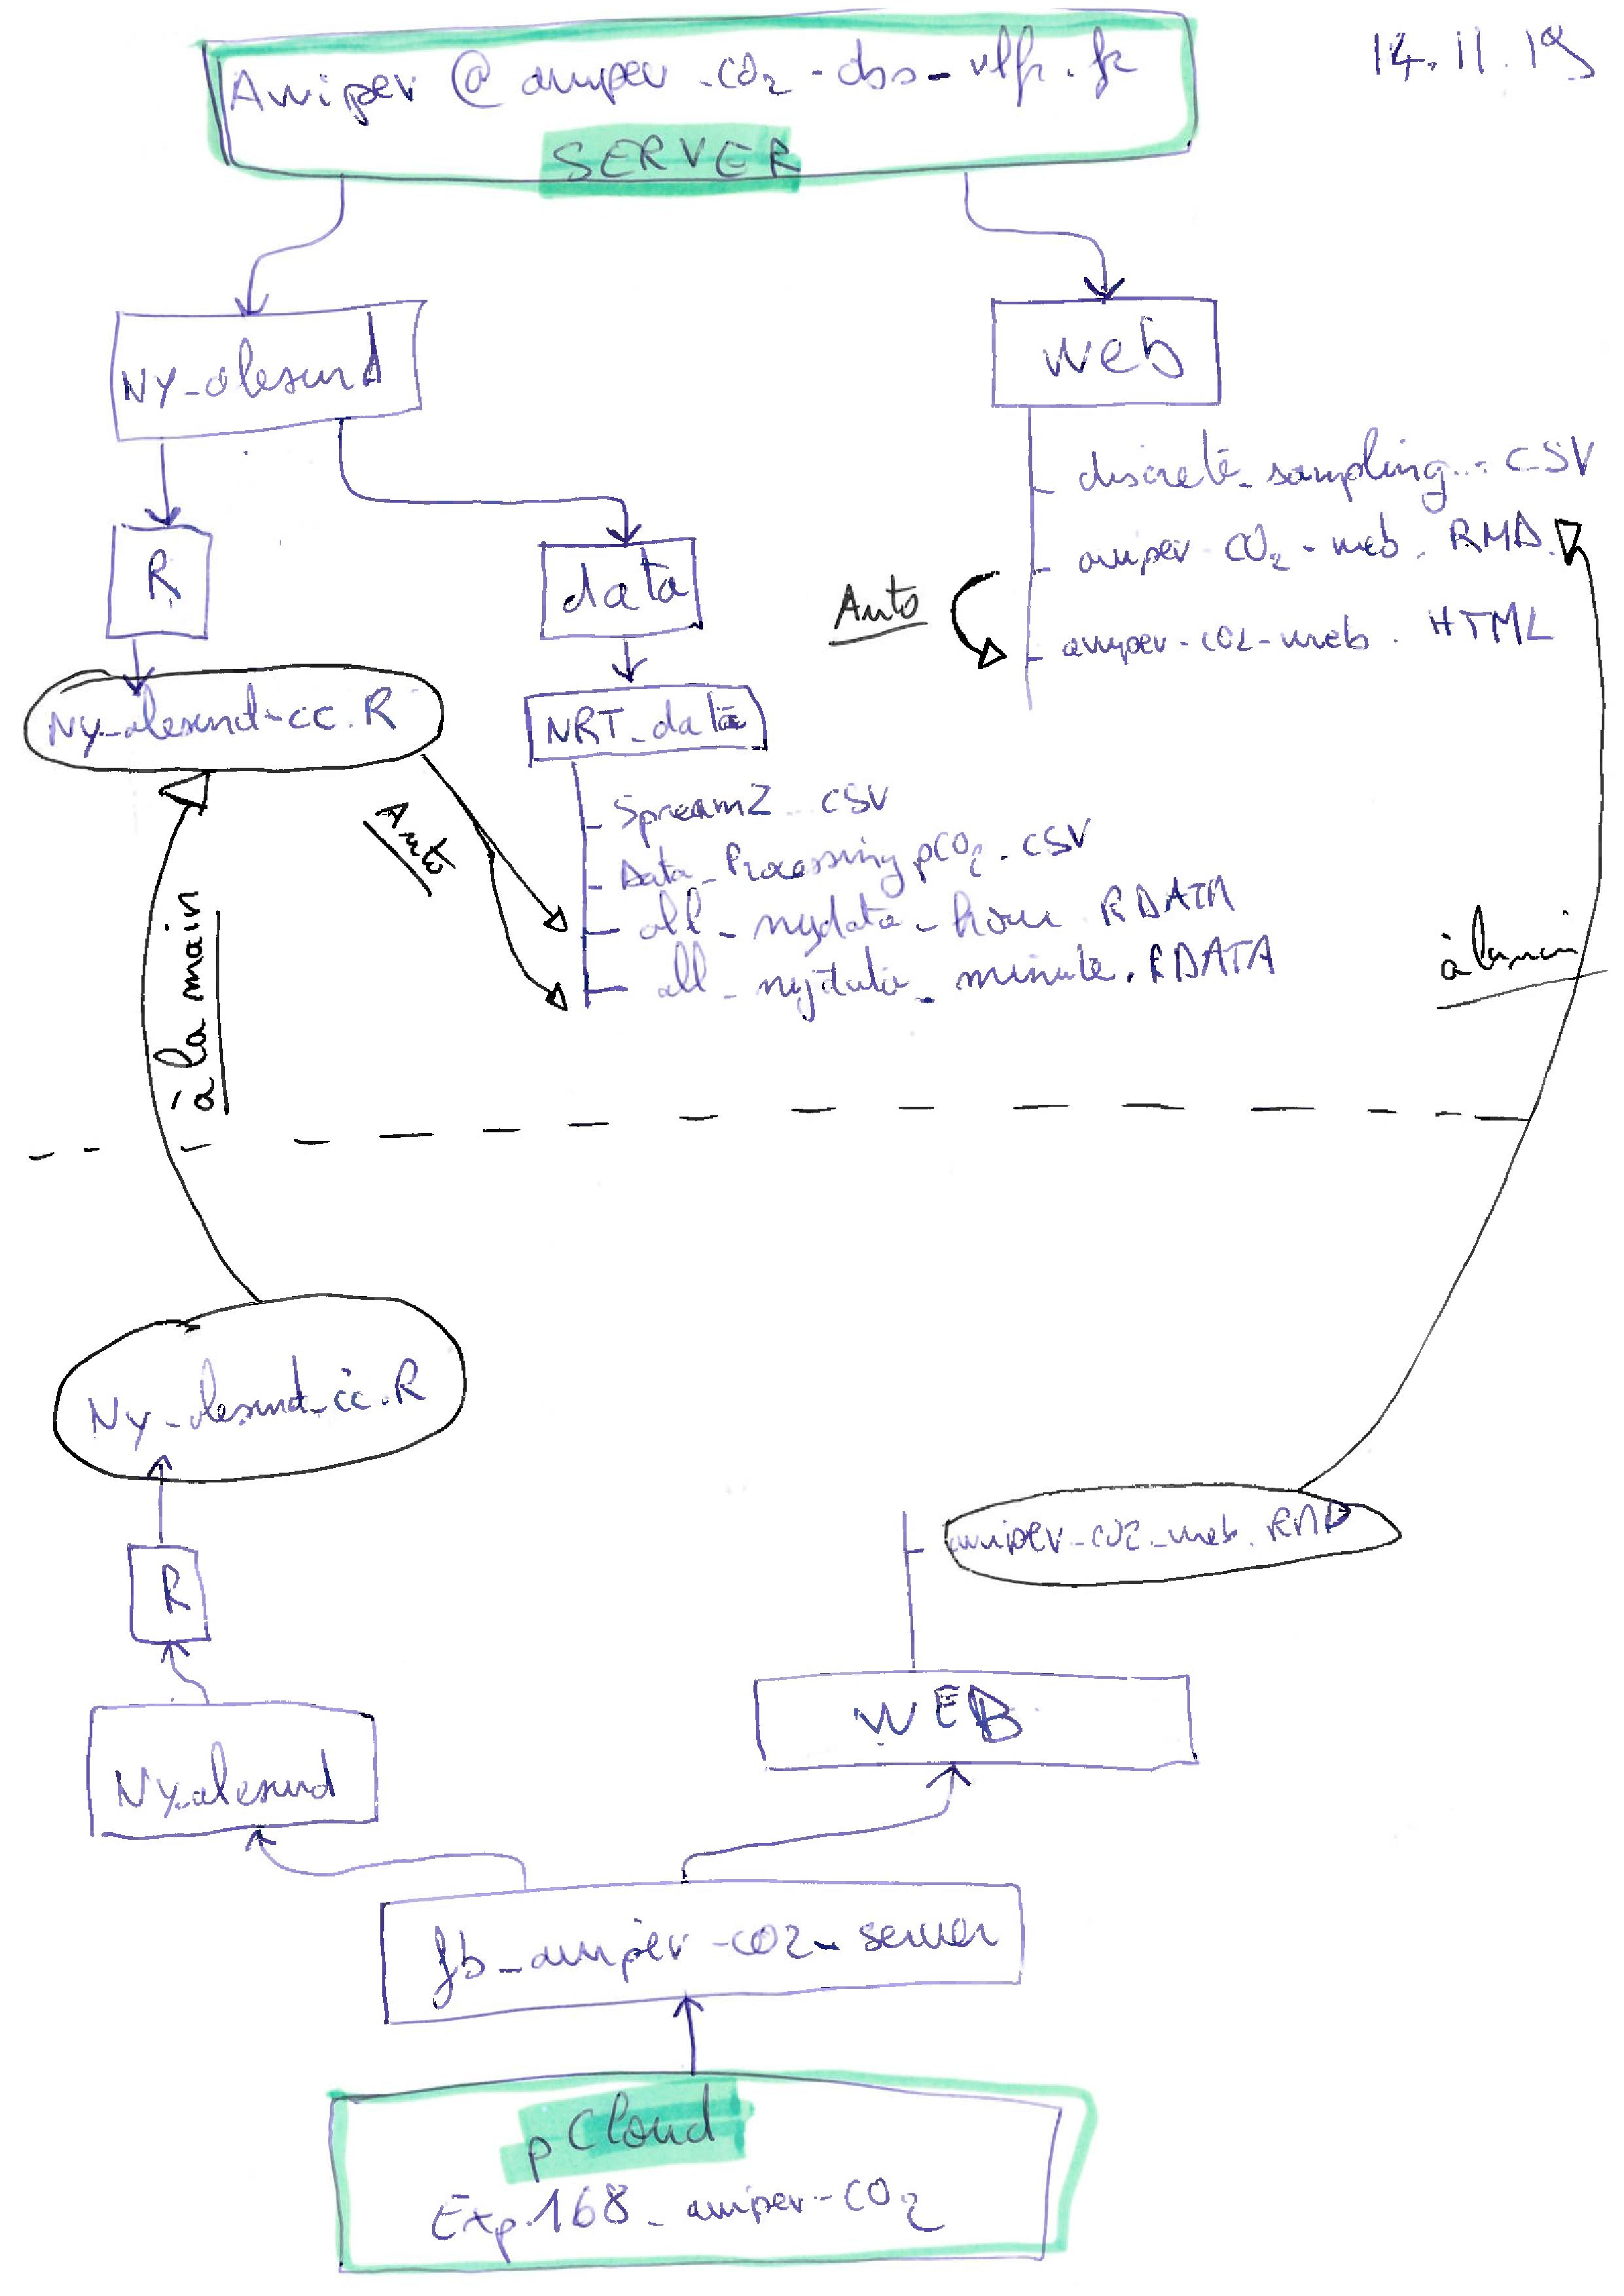
\includegraphics[width=0.65\textwidth,height=\textheight]{Images/awipev_server_arborescence.jpg}

\end{document}
